\chapter{Reglas aritméticas}\label{subseccion_reglas_aritmeticas}

\section{Orden de la recta}\label{subsubsection_orden_de_la_recta}

Los números que usualmente utilizamos para contar 
\[
			\left\{1,2,3,4,\dots,100,101,102,\dots \right\}
\]
son llamados \textbf{números naturales}.. 

Hay otra familia de números que nos ayudan a representar medidas negativas y son llamados los \textbf{números negativos}. Por ejemplo, en un térmometro las temperaturas por debajo de $0\degree$ son temperaturas negativas.

Juntando los números naturales, los negativos y el cero obtenemos los \textbf{números enteros}, que se pueden organizar en una recta númerica:

		\begin{figure}[H]
			\centering
			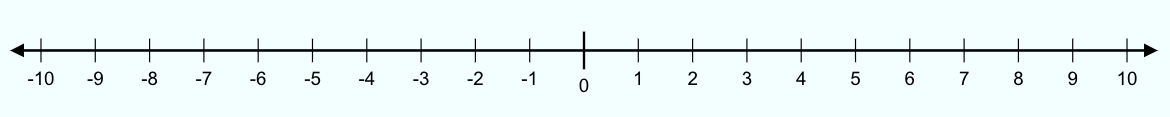
\includegraphics[width=0.7\linewidth]{Algebra/imgs/recta_numerica}
			\caption{}
			\label{rectanumerica}
		\end{figure}
	
\begin{itemize}
			\item Entrar a \url{https://phet.colorado.edu/es/simulation/number-line-integers} para experimentar ubicando números enteros.
			\item Una vez conocemos la ubicación de los números podemos compararlos. Quien es mayor, quien es menor.
\end{itemize}

\begin{exer}
	Discuta cuando los sigueintes números existen. Si existen, diga su valor.
	\begin{enumerate}[label=\Alph*)]
		\item El mayor entero positivo.
		\item Elmenos entero positivo.
		\item El mayor entero negativo.
		\item El menor entero negativo.
	\end{enumerate}
\end{exer}

\begin{ejemplo}
(8 pag 119 de \cite{Dimensions_Math_6A}). Considere la suma
\[
			1-1+1-1+1-1\cdots,
\]
así sucesivamente alternando $+1$ y $-1$. La suma de los primeros dos términos es $1-1=0$.
		\begin{enumerate}[label=\Alph*)]
					\item Encontrar la suma de los primeros 10 términos.
					\item Encontrar la suma de los primeros 15 términos.
					\item Encontrar la suma de los primeros 231 términos.						
		\end{enumerate}
\textbf{Rta: }	Se puede hacer primero algebraicamente y después geométricamente, mostrando que voy saltando hacia adelante y atras en la recta, que cuando es impar quedo en 1 y cuando es par quedo en 0.
\end{ejemplo}

En la recta también podemos ubicarlos \textbf{números racionales} es decir, las fracciones. Y los \textbf{números reales } que son básicamente los números decimales.
\begin{ejemplo}
Abrir geogebra, quitar el fondo, la cuadricula y el eje $y$. Luego ubicar los números números:
\begin{multicols}{2}
		\begin{enumerate}[label=\Alph*)]
				\item $\frac{1}{2}$
				\item $-\frac{3}{2}$
				\item $12.5$
				\item $-0.35$
				\item $1.5$
				\item $-1\frac{1}{4}$
		\end{enumerate}
\end{multicols}
Ordenarlos de menor a mayor.
\end{ejemplo}

\newpage
\begin{center}
	\vspace{-1cm}
	\subsection{ Orden de la recta}\label{ejercicios_subsubsection_orden_de_la_recta}
\end{center}
\begin{enumerate}
		\item Ordenar de forma ascendente los números: $12,-12,0,6\frac{2}{3}$.
		\item Ordenar de forma decreciente los números: $8.5,5,0,-4\frac{1}{2}$.
		\item (11 pag 127 de \cite{Dimensions_Math_6A}). En una Olimpiada matemática consta de cinco preguntas. Por cada respuesta correcta el concursante obtiene 3 puntos, por cada incorrecta $-2$ puntos y por cada no contestada $0$ puntos.
				\begin{enumerate}[label=\Alph*)]
						\item Cuánto es el máximo puntaje?
						\item Cuánto es el mínimo puntaje ?
						\item Escriba la mayor cantidad de situaciones posibles en las que el estudiante puede obtener 4 puntos.
						\item Escriba la mayor cantidad de situaciones posibles en las que el estudiante puede obtener -5 puntos.
				\end{enumerate}
\end{enumerate} 
\newpage

\section{Operaciones entre números reales}\label{subsubsection_operaciones_entre_numeros_reales}

\subsection{Adición}\label{subsubsubsection_adicion_numeros_reales}

En la recta la \textbf{adición de un número positivos} se representa con un movimiento \textit{hacia la derecha}. Y la \textbf{adición de números negativos} se presenta con un movimiento \textit{hacia la izquierda}. Veamos unos ejemplos.

\begin{ejemplo}
	(p.33 de \cite{Dimensions_Math_7A})
	\begin{itemize}
			\item Veamos cuánto es $(-3)+4$
					\begin{figure}[H]
						\centering
						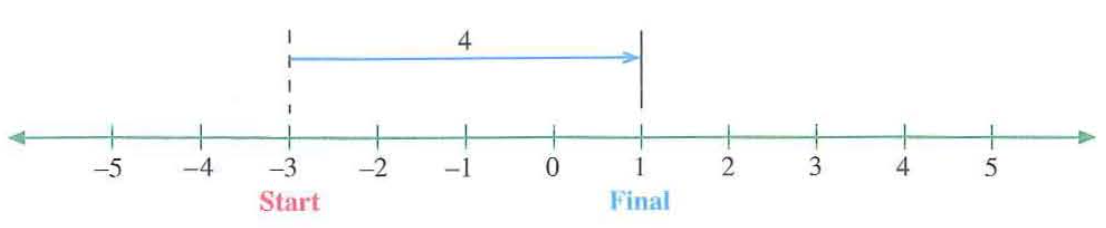
\includegraphics[width=0.7\linewidth]{Algebra/imgs/DM7A_p33_1a}
						%\caption{}
						\label{DM7A_p33_1a}
					\end{figure}
			\item Veamos cuánto es $2+3$
					\begin{figure}[H]
						\centering
						\includegraphics[width=0.7\linewidth]{Algebra/imgs/DM7A_p33_1B}
						%\caption{}
						\label{DM7A_p33_1B}
					\end{figure}
			\item Veamos cuánto es $(-1)+(-3)$
					\begin{figure}[H]
						\centering
						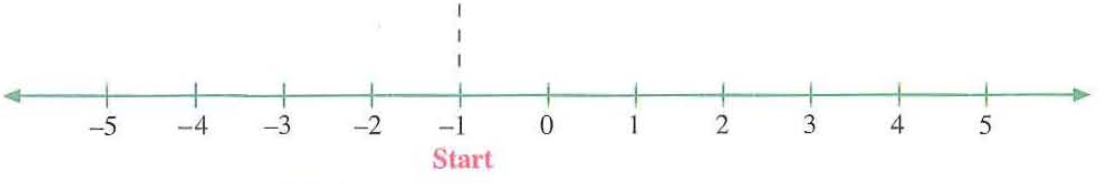
\includegraphics[width=0.7\linewidth]{Algebra/imgs/DM7A_p33_2a}
						%\caption{}
						\label{DM7A_p33_2a}
					\end{figure}
			\item Veamos cuánto es $2+(-5)$		
					\begin{figure}[H]
						\centering
						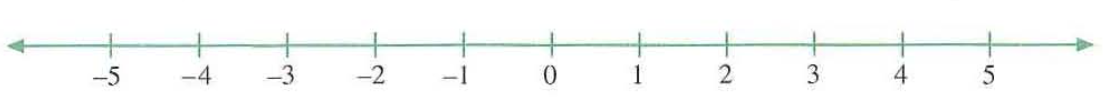
\includegraphics[width=0.7\linewidth]{Algebra/imgs/DM7A_p33_2b}
						%\caption{}
						\label{DM7A_p33_2b}
					\end{figure}
			\item Veamos cuánto es $0+(-4)$		
					\begin{figure}[H]
						\centering
						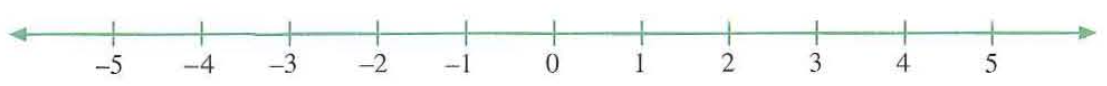
\includegraphics[width=0.7\linewidth]{Algebra/imgs/DM7A_p33_2c}
						%\caption{}
						\label{DM7A_p33_2c}
					\end{figure}					
	\end{itemize}
\end{ejemplo}

\begin{exer}
	(p.35 de \cite{Dimensions_Math_7A}). Encontrar el valor de 
	\begin{multicols}{3}
		\begin{enumerate}[label=\Alph*)]
				\item $13+(-6)$
				\item $(-25)+9$
				\item $(-11)+(-4)$
				\item $9+(-20)$
				\item $(-6)+14$
				\item $(-8)+(-13)$
		\end{enumerate}
	\end{multicols}
\end{exer}

Vemos entonces que sumar números negativos es lo mismo que sumar números positivos, es decir
\[
		(-a)+(-b)=-(a+b).
\]

Todo número real tiene un \textbf{inverso aditivo}, el cuál es el número que al sumarlo con el número que tenía me da cero. Por ejemplo el inverso de $(-3)$ es $\color{red}3$ porque $(-3)+\color{red}3\color{black}=0$.

\begin{ejemplo}
		(p.36 de \cite{Dimensions_Math_7A})
		\begin{itemize}
				\item El inverso de $-4$ es el $4$.
				\item El inverso de $-18$ es el $18$.
				\item El inverso de $620$ es el $-620$.								
		\end{itemize}
\end{ejemplo}

\begin{exer}
	(p.36 de \cite{Dimensions_Math_7A}). Encontrar el inverso aditivo de 
	\begin{multicols}{3}
		\begin{enumerate}[label=\Alph*)]
			\item $60$
			\item $-244$
			\item $-8.921$
		\end{enumerate}
	\end{multicols}
\end{exer}

\newpage

\begin{center}
	\vspace{-1cm}
	\subsubsection{Ejercicios: Adición}\label{ejercicios_subsubsection_adicion_numeros_reales}
\end{center}
\begin{enumerate}
		\item (2 pag 37 de \cite{Dimensions_Math_7A}). Calcular las siguientes sumas
				\begin{multicols}{3}
						\begin{enumerate}[label=\Alph*)]
								\item $(-5)+7$.
								\item $(-12)+(-25)$.
								\item $24+(-30)$.
								\item $(-60)+28$.
								\item $-46+(-54)$.
								\item $-13+79$.
						\end{enumerate}	
				\end{multicols}
		
		\item (5 pag 37 de \cite{Dimensions_Math_7A}). Completar para que la igualdad sea cierta.
		\begin{multicols}{3}
			\begin{enumerate}[label=\Alph*)]
				\item $\rule{5mm}{0.15mm}+ 7 = 3$.
				\item $ 11 + \rule{5mm}{0.15mm} = -5$.
				\item $ -8 + \rule{5mm}{0.15mm} = 6$.
				\item $ \rule{5mm}{0.15mm} + (-13)= -14$.
			\end{enumerate}	
		\end{multicols}
		
		\item Calcular
				\[
						\underbrace{(-2)+(-2)+(-2)+\cdots+(-2)}_{50 \text{ veces}}
				\] 
				
		\item Calcular
				\[
						1+(-2)+3+(-4)+5+(-6)+7\cdots + 97+(-98)+99
				\]
				
		\item Hay 7 enteros consecutivos que al sumarlos todos de 0?
		
		\item Tengo una lista de enteros consecutivos de tal forma que suman 10. Cuánto es la mayor cantidad de enteros que puede tener esa lista?
\end{enumerate}
\newpage

\subsection{Resta}\label{subsubsubsection_resta_numeros_reales}
En la recta la \textbf{resta de un número positivo} se representa con un movimiento \textit{hacia la izquierda}. Y la \textbf{resta de un número negativo} se presenta con un movimiento \textit{hacia la derecha}. Veamos unos ejemplos.

\begin{ejemplo}
(p.38 de \cite{Dimensions_Math_7A})
	\begin{itemize}
		\item Veamos cuánto es $3-4$
				\begin{figure}[H]
					\centering
					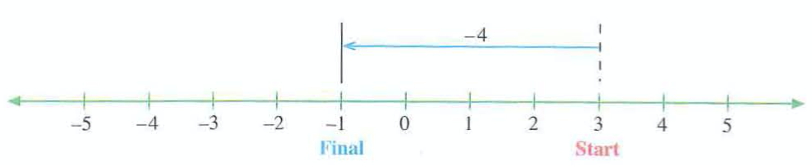
\includegraphics[width=0.7\linewidth]{Algebra/imgs/DM7A_p38_1a}
					%\caption{}
					\label{DM7A_p38_1a}
				\end{figure}
		\item Veamos cuánto es $-2-3$
				\begin{figure}[H]
					\centering
					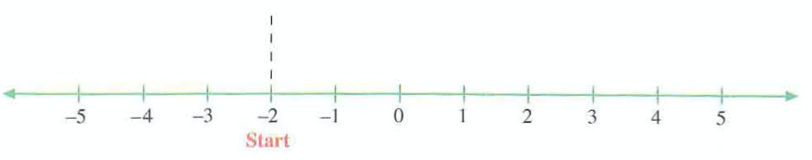
\includegraphics[width=0.7\linewidth]{Algebra/imgs/DM7A_p38_1b}
					%\caption{}
					\label{DM7A_p38_1b}
				\end{figure}
		\item Veamos cuánto es $(-1)-(-3)$
				\begin{figure}[H]
					\centering
					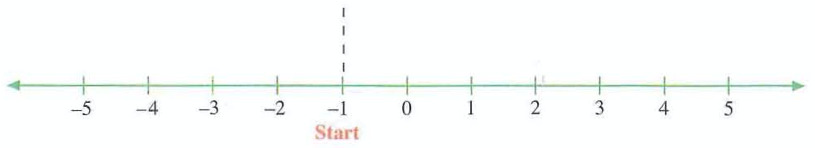
\includegraphics[width=0.7\linewidth]{Algebra/imgs/DM7A_p38_2a}
					%\caption{}
					\label{DM7A_p38_2a}
				\end{figure}
		\item Veamos cuánto es $2-(-2)$		
				\begin{figure}[H]
					\centering
					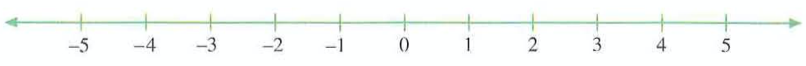
\includegraphics[width=0.7\linewidth]{Algebra/imgs/DM7A_p38_2b}
					%\caption{}
					\label{DM7A_p38_2b}
				\end{figure}
		\item Veamos cuánto es $0-(-5)$		
				\begin{figure}[H]
					\centering
					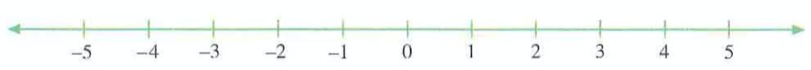
\includegraphics[width=0.7\linewidth]{Algebra/imgs/DM7A_p38_2c}
					%\caption{}
					\label{DM7A_p38_2c}
				\end{figure}					
	\end{itemize}
\end{ejemplo}

\begin{ejemplo}
(p.37 de \cite{Dimensions_Math_7A}). Con ayuda de la recta
		\begin{figure}[H]
			\centering
			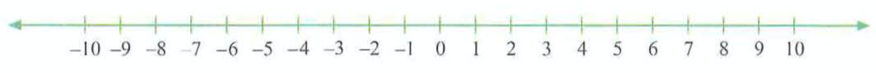
\includegraphics[width=0.7\linewidth]{Algebra/imgs/recta_numerica_larga}
			\caption{Recta numérica}
			\label{recta_numerica_larga}
		\end{figure}
Complete la siguiente tabla 
		\begin{figure}[H]
			\centering
			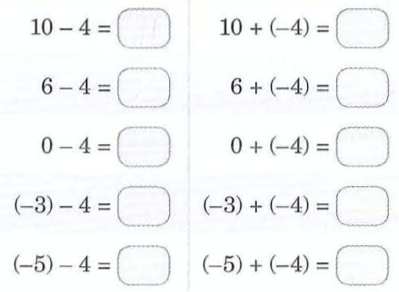
\includegraphics[width=0.5\linewidth]{Algebra/imgs/DM7A_p39_3a}
			\caption{}
			\label{DM7A_p39_3a}
		\end{figure}
\end{ejemplo}

De acá podemos concluir que 
\[
		a-b=a+(-b)
\]

\begin{ejemplo}
	(p.37 de \cite{Dimensions_Math_7A}). Con ayuda de la recta numérica de la figura \ref{recta_numerica_larga} complete la siguiente tabla 
	\begin{figure}[H]
		\centering
		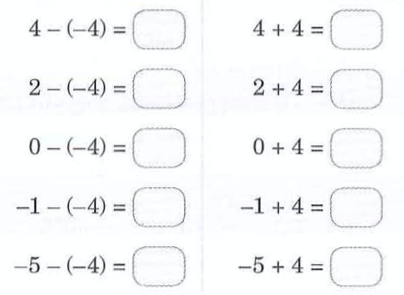
\includegraphics[width=0.5\linewidth]{Algebra/imgs/DM7A_p39_3b}
		\caption{}
		\label{DM7A_p39_3b}
	\end{figure}
\end{ejemplo}

De acá podemos concluir que 
\[
a-(-b)=a+b
\]

\begin{exer}
	(p.40 de \cite{Dimensions_Math_7A}). Encontrar el valor de 
	\begin{multicols}{3}
		\begin{enumerate}[label=\Alph*)]
			\item $12-23$
			\item $-16-(-9)$
			\item $0-(-17)$
			\item $15-28$
			\item $-12-(-4)$
			\item $3-(-10)$
		\end{enumerate}
	\end{multicols}
\end{exer}

\newpage

\begin{center}
	\vspace{-1cm}
	\subsubsection{Ejercicios: Resta}\label{ejercicios_subsubsection_resta_numeros_reales}
\end{center}
\begin{enumerate}
	\item (2 pag 43 de \cite{Dimensions_Math_7A}). Calcular las siguientes restas
	\begin{multicols}{3}
		\begin{enumerate}[label=\Alph*)]
			\item $7-16$.
			\item $0-20$.
			\item $3-(-32)$.
			\item $-9-15$.
			\item $-4-(-18)$.
			\item $-28-(-11)$.
		\end{enumerate}	
	\end{multicols}
	
	\item (3 pag 43 de \cite{Dimensions_Math_7A}). Completar para que la igualdad sea cierta.
	\begin{multicols}{3}
		\begin{enumerate}[label=\Alph*)]
			\item $5 - \rule{5mm}{0.15mm}= 12$.
			\item $ 7-  \rule{5mm}{0.15mm} = -13$.
			\item $ -9 + \rule{5mm}{0.15mm} = -15$.
			\item $ -8-\rule{5mm}{0.15mm} = -10$.
		\end{enumerate}	
	\end{multicols}
	
	
	\item Calcular
	\[
	-1-(-2)-3-(-4)-5-(-6)-7\cdots - 97-(-98)-99
	\]			
\end{enumerate}
\newpage

\newpage

\begin{center}
	\vspace{-1cm}
	\subsection{ Ejercicios: Relevos con problemas de Sumas y restas }\label{ejercicios:subsubsection:restaNumerosReales:relevos1}
\end{center}

\begin{center}
\textbf{Competencia  1 de relevos}
\end{center}
\textbf{Lee antes de empezar! } Hola Mate amigo, Bienvenido a la prueba de relevos!, te explico: Cada problema tiene un ejercicio, el cuál debes solucionar y tiene como respuesta un número, esa respuesta la debes utilizar para el siguiente problema y así sucesivamente hasta responder todos los problemas. Si todos los problemas quedaron bien, la respuesta del último problema debe estar bien entonces, esa será la respuesta que enviarán como solución de esta \textbf{competencia 1 de relevos}.
\vspace{1cm}
\begin{enumerate}
	\item Cuánto es $5+17$?
	
	\item En el espacio va la respuesta del problema anterior. Cuánto es $\rule{5mm}{0.15mm} - 20?$
	
	\item En el espacio va la respuesta del problema anterior. Cuánto es $-4-\rule{5mm}{0.15mm} ?$
	
	\item Cúanto debemos sumarle a la respuesta del problema anterior para que nos de $4$?
	
	\item Cúanto debemos restarle a la respuesta del problema anterior para que nos de $-30$?
	
	\item En el espacio va la respuesta del problema anterior. Cuánto es $-4-\rule{5mm}{0.15mm} ?$
\end{enumerate}

\textbf{Terminaste! } Dile a tu profesor el resultado que obtuviste al final en este relevo.
\newpage

\begin{center}
	\textbf{Competencia  2 de relevos}
\end{center}
	
\textbf{Lee antes de empezar! } Hola Mate amigo, Bienvenido a la prueba de relevos!, te explico: Cada problema tiene un ejercicio, el cuál debes solucionar y tiene como respuesta un número, esa respuesta la debes utilizar para el siguiente problema y así sucesivamente hasta responder todos los problemas. Si todos los problemas quedaron bien, la respuesta del último problema debe estar bien entonces, esa será la respuesta que enviarán como solución de esta \textbf{competencia 1 de relevos}.
\vspace{1cm}
\begin{enumerate}
	\item Cuánto es $13+15$?
	
	\item En el espacio va la respuesta del problema anterior. Cuánto es $\rule{5mm}{0.15mm} - 30?$
	
	\item En el espacio va la respuesta del problema anterior. Cuánto es $-4-\rule{5mm}{0.15mm} ?$
	
	\item Cúanto debemos sumarle a la respuesta del problema anterior para que nos de $12$?
	
	\item Cúanto debemos restarle a la respuesta del problema anterior para que nos de $-15$?
	
	\item En el espacio va la respuesta del problema anterior. Cuánto es $30-\rule{5mm}{0.15mm} ?$
\end{enumerate}

\textbf{Terminaste! } Dile a tu profesor el resultado que obtuviste al final en este relevo.
\newpage

\begin{center}
	\textbf{Competencia  3 de relevos}
\end{center}
	
\textbf{Lee antes de empezar! } Hola Mate amigo, Bienvenido a la prueba de relevos!, te explico: Cada problema tiene un ejercicio, el cuál debes solucionar y tiene como respuesta un número, esa respuesta la debes utilizar para el siguiente problema y así sucesivamente hasta responder todos los problemas. Si todos los problemas quedaron bien, la respuesta del último problema debe estar bien entonces, esa será la respuesta que enviarán como solución de esta \textbf{competencia 1 de relevos}.
\vspace{1cm}
\begin{enumerate}
	\item Cuánto es $(-2)+(-2)+(-2)+(-2)$?
	
	\item En el espacio va la respuesta del problema anterior. Cuánto es $\rule{5mm}{0.15mm} + 10?$
	
	\item En el espacio va la respuesta del problema anterior. Cuánto es $-\rule{5mm}{0.15mm} - 3?$
	
	\item Cúanto debemos sumarle a la respuesta del problema anterior para que nos de $12$?
	
	\item Cúanto debemos restarle a la respuesta del problema anterior para que nos de $20$?
	
	\item En el espacio va la respuesta del problema anterior. Cuánto es $\rule{5mm}{0.15mm} - (-6)?$
	
	\item Cuánto debemos sumarle a la respuesta anterior para que nos de $1$
	
\end{enumerate}

\textbf{Terminaste! } Dile a tu profesor el resultado que obtuviste al final en este relevo.
\newpage


\subsection{Producto y división}\label{subsubsubsection_producto_numeros_reales}

El producto es normal, solo hay que tener en cuenta los signos.
\[
		a(-b) = -ab,
\]
y
\[
		(-a)(-b)=ab.
\]
Es decir
\begin{itemize}
		\item Si tienen el \textbf{mismo signo} entonces el \textbf{producto es positivo}.
		\item Si tienen \textbf{diferente signo} entonces el \textbf{producto es negativo}. 
\end{itemize}

\begin{ejemplo}
	(p.47 de \cite{Dimensions_Math_7A}). Evaluar los siguientes productos:
			\begin{multicols}{3}
					\begin{enumerate}[label=\Alph*)]
						\item $(-6)\times 9 $.
						\item $(-4)\times (-4)$.
						\item $8\times (-4)\times (-7)$
					\end{enumerate}	
			\end{multicols}
\end{ejemplo}

\begin{exer}
	(p.47 de \cite{Dimensions_Math_7A}). Evaluar los siguientes productos:
	\begin{multicols}{3}
		\begin{enumerate}[label=\Alph*)]
			\item $8\times (-12)$.
			\item $(-3)\times (-6)$.
			\item $(-5)\times 6\times (-4)$
		\end{enumerate}	
	\end{multicols}
\end{exer}

Recordemos que 
\[
		{(-2)}^3=\underbrace{(-2)\times (-2)\times (-2)}_{3 \textit{ veces}} = -8
\]

\begin{exer}
Evaluar los siguientes productos:
	\begin{multicols}{3}
		\begin{enumerate}[label=\Alph*)]
			\item $3^3$.
			\item ${(-4)}^2$.
			\item ${(-5)}^3$.
			\item $(-2)\times {(-6)}^2$.
			\item ${(-3)}^2\times {(-2)}^5$.
			\item ${(-1)}^{100}$.
		\end{enumerate}	
	\end{multicols}
\end{exer}

Para la división se aplica la misma regla. 
\[
\frac{a}{(-b)} = -\frac{a}{b}\quad \text{ ó } \quad \frac{(-a)}{b} = -\frac{a}{b}
\]
y
\[
\frac{(-a)}{(-b)}=\frac{a}{b}.
\]
Es decir
\begin{itemize}
	\item Si tienen el \textbf{mismo signo} entonces el \textbf{cociente es positivo}.
	\item Si tienen \textbf{diferente signo} entonces el \textbf{cociente es negativo}. 
\end{itemize}

\begin{ejemplo}
	(p.48 de \cite{Dimensions_Math_7A}). Evaluar los siguientes cocientes:
	\begin{multicols}{3}
		\begin{enumerate}[label=\Alph*)]
			\item $\frac{(-42)}{(-7)} $.
			\item $\frac{(-36)}{(3)} $.
			\item $\frac{14}{(-7)} $.						
		\end{enumerate}	
	\end{multicols}
\end{ejemplo}

\begin{exer}
	(p.48 de \cite{Dimensions_Math_7A}). Evaluar los siguientes productos:
	\begin{multicols}{3}
		\begin{enumerate}[label=\Alph*)]
			\item $\frac{54}{(-6)} $.
			\item $\frac{(-75)}{(-5)} $.			
			\item $\frac{33}{(-11)} $.			
		\end{enumerate}	
	\end{multicols}
\end{exer}

\section{Orden de las operaciones}\label{subsubsection_orden_de_las_operaciones}
Que significa cuando escribimos por ejemplo
\[
		2+3\times 4?
\]
Significa 
\[
		\textit{ Sumar 2 y 3 y luego multiplicar por 4? } \equiv 6\times 4=24
\]
o significa 
\[
\textit{ multiplicar 3 por 4 y luego sumar 2? } \equiv 2+12=14.
\]

\begin{tcolorbox}[colback=red!5!white,colframe=red!75!black]
	Para evitar estas confusiones hay unas reglas para tener \textbf{orden en las operaciones}. Estas son
	\begin{enumerate}
		\item Si hay paréntesis en la expresión, evaluar primero los paréntesis de adentro hacia afuera. Haga las operaciones dentro de los parentesis teniendo en cuenta el orden de las operaciones.
		\item Resolver las potencias.
		\item Resolver todas las multiplicaciones y divisiones de izquierda a derecha.
		\item Resolver todas las sumas y restas de izquierda a derecha.
	\end{enumerate}
\end{tcolorbox}


Veamos unos ejemplos:
\begin{ejemplo}
		\begin{enumerate}
		\item 	
			\begin{align*}
					5+3\times 6^2	&= 5+3\times 36 & &\text{(Potencias)}\\
												&= 5+108 & &\text{(Multiplicación)}\\
												&= 113 & &\text{(Suma)}
			\end{align*}
		\item 	Si queremos hacer primero la suma de $5$ y $3$ que debemos hacer? \textbf{Rta:}
			\begin{align*}
			\color{red}(\color{black}5+3\color{red})\color{black}\times 6^2	&= 8\times 6^2 & &\text{(Paréntesis)}\\
			&= 8+36 & &\text{(Potencia)}\\
			&= 44 & &\text{(Suma)}
			\end{align*}
		\end{enumerate}
\end{ejemplo}

\begin{ejemplo}
	(p.4 de \cite{Aops_algebra}). Evaluar las siguientes expresiones teniendo en cuenta el orden de las operaciones:
	\begin{multicols}{2}
		\begin{enumerate}[label=\Alph*)]
			\item $6+3\times 8$.
			\item $(6+3)\times 8$.
			\item $17-2\times 3^2$.	
			\item $17 - {(2\times 3)}^2$.
			\item ${(17-2\times 3)}^2$.
			\item $\left[ (15-3)/2 \right]\times 3 - (2^2\times 3)/6$.					
		\end{enumerate}	
	\end{multicols}
\end{ejemplo}

\newpage

\begin{center}
	\vspace{-1cm}
	\subsection{ Ejercicios: Orden de las operaciones}\label{ejercicios_subsubsection_orden_de_las_operaciones}
\end{center}

\begin{enumerate}
\item (p.4 de \cite{Aops_algebra}). Evaluar las siguientes expresiones teniendo en cuenta el orden de las operaciones:
		\begin{multicols}{3}
		\begin{enumerate}[label=\Alph*)]
				\item $3^2 +4\times 2$.
				\item $(5-8)\times (2+7)$.
				\item $(3^3-5^2)\times 5 - 8$.	
				\item $8/(6-2)+5$.
				\item $8^2/4^2+3\times 4$.
				\item $11\times 6^{(2^2-3)}$.					
		\end{enumerate}	
		\end{multicols}
\item (p.50 de \cite{Dimensions_Math_7A}). Evaluar las siguientes expresiones
		\begin{multicols}{2}
		\begin{enumerate}[label=\Alph*)]
				\item $(-6)\times 3\times (-1)$.
				\item $(-84)/7\times 5$.
				\item $(-37)\times 0 - (-8)$.	
				\item $63/(-9)+(-2)\times (-10)$.
				\item $(-47)-33/(-3)-3\times(-7)$.
				\item $196/\left[ (-8) + (-6) \right]\times (-2)$.	
				\item $\left[(-23)+14\right]\times {(-2)}^2$.	
				\item $(-45)\times 6/{(-3)}^3$.
				\item $(-7)\times(-8)\times 0\times 34 - 4 \times {(-5)}^2$.
				\item ${(-6)}^3/3^2/{\left[-9-(-8)\right]}^3$.			
		\end{enumerate}	
		\end{multicols}
\item (Udea clasificatoria 2020). Si tomamos $b=-3$,cuál es el mayor número del siguiente conjunto ?
\[
\left\{	-9b, 4b, \frac{-27}{b}, b^2, 18	\right\}
\]
\end{enumerate}
\newpage

\section{Conmutatividad de las operaciones: suma, multiplicación, resta y división }\label{subsubsection_conmutatividad_de_operaciones}

\begin{ejemplo}
		A continuación decir si la igualdad es Verdadera o Falsa:
		\begin{multicols}{2}
		\begin{enumerate}[label=\Alph*)]
				\item $14+8=8+14$.
				\item $53+81=81+53$.
				\item $8+(-4)=(-4)+8$.
				\item $\frac{1}{5} + \frac{6}{7} = \frac{6}{7} + \frac{1}{5}$.
		\end{enumerate}
		\end{multicols}
\end{ejemplo}

\begin{tcolorbox}[colback=red!5!white,colframe=red!75!black]
	\begin{itemize}
		\item \textbf{La suma cumple la propiedad conmutativa} esto es:
		\[
		\textit{La suma de dos números es la misma sin importar el orden en que se sume}
		\]
		Esto mismo lo podemos decir de otra forma para no decirlo en palabras. Para esto como se cumple para cuales quiera números, vamos a usar letras (llamadas \textbf{variables}) para representar los números y así la propiedad conmutativa de la suma sería:
		\[
		a+b=b+a
		\]
		En el caso por ejemplo en el que $a=14$ y $b=8$, tenemos que 
		\[
		14+8=8+14
		\]
	\end{itemize}
\end{tcolorbox}


\begin{ejemplo}\label{pro1_3_aopsalg} (p.7 de \cite{Aops_algebra}). Juana y René están contando las baldosas de la sala. El piso de la sala es el siguiente
		\begin{figure}[H]
			\centering
			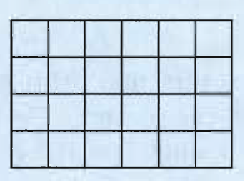
\includegraphics[width=0.5\linewidth]{Algebra/imgs/AopsALG_pag7_p1_3}
			\caption{Piso de la sala, Ejemplo \ref{pro1_3_aopsalg}}
			\label{AopsALG_pag7_p1_3}
		\end{figure}
Juana dice 
\[
		\textit{Hay 6 columnas y 4 filas, entonces en total hay $6\times 4$ baldosas}.
\]
Mientras que René dice
\[
\textit{Hay 4 filas y 6 columnas,, entonces en total hay $4\times 6$ baldosas}.
\]
Quién tiene la razón?\\
\textbf{Rta: }Ambas porque $6\times 4=4\times 6$.
\end{ejemplo}

Esto siempre se cumplirá? veamos el siguiente ejemplo.
\begin{ejemplo}
	A continuación decir si la igualdad es Verdadera o Falsa:
	\begin{multicols}{2}
		\begin{enumerate}[label=\Alph*)]
			\item $12\times 8=8\times 12$.
			\item $1.5\times 3=3\times 1.5$.
			\item $2\times(-4)=(-4)\times 2$.
			\item $\frac{1}{2}\times  \frac{5}{3} = \frac{5}{3} + \frac{1}{2}$.
			\item $3.5 \times  \frac{1}{8} = \frac{1}{8} \times 3.5$.			
			\item $(-0.5) \times  \frac{6}{(-5)} = \frac{6}{(-5)} \times (-0.5)$.			
		\end{enumerate}
	\end{multicols}
\end{ejemplo}


\begin{tcolorbox}[colback=red!5!white,colframe=red!75!black]
	\begin{itemize}
		\item \textbf{La multiplicación cumple la propiedad conmutativa} esto es:
		\[
		\textit{El producto de dos números es el mismo sin importar el orden en que se multiplique}
		\]
		Usando variables esto se puede decir de la siguiente forma
		\[
		a\times b=b\times a
		\]
		En el caso por ejemplo en el que $a=2$ y $b=3$, tenemos que 
		\[
		2\times 3=3\times 2
		\]
	\end{itemize}
\end{tcolorbox}



\begin{ejemplo}
		A continuación decir si la igualdad es Verdadera o Falsa:
		\begin{multicols}{2}
		\begin{enumerate}[label=\Alph*)]
				\item $2-5=5-2$.
				\item $2+(-5)=(-5)+2$.
				\item $8/4=4/8$.
				\item $8\times \frac{1}{4} = \frac{1}{4} \times 8$		
		\end{enumerate}
		\end{multicols}
	
		\textbf{Rta: } Veamos por orden.
		\begin{enumerate}[label=\Alph*)]
				\item $2-5=-3$ y $5-2=3$. Entonces es Falsa porque $3\neq -3$. Entonces será que la \textbf{ley conmutativa se cumple con la resta}? \color{red} NO. \color{black}, para probar que algo no es siempre cierto basta encontrar un caso que no cumpla.
				\item $2+(-5)=-3$ y $(-5)+2=-3$. Entonces es Verdadero. Además como la suma es conmutativa, ya sabíamos que esto era verdadero.
				\item $8/4=2$ y $4/8=\frac{1}{2}$. Entonces es Falsa porque $2\neq \frac{1}{2}$. Entonces será que la \textbf{ley conmutativa se cumple con la división}? \color{red} NO. \color{black}
				\item $8\times \frac{1}{4} = 2$ y $\frac{1}{4} \times 8=2$. Entonces es Verdadero. Además como la multiplicación es conmutativa, ya sabíamos que esto era verdadero.	
		\end{enumerate}
\end{ejemplo}

De este ejemplo tenemos entonces que:
\begin{itemize}
	\item \textbf{La resta y la división \color{red} NO \color{black} cumplen con la propiedad conmutativa}.
\end{itemize}

\begin{exer}
		Dar 3 ejemplos donde se evidencie que la resta no es conmutativa y 3 ejemplos donde se evidencie que la división no es conmutativa.
\end{exer}

Entonces en la suma y en la multiplicación podemos reacomodar los números como queramos, veamos mas ejemplos.

\begin{ejemplo}{\ \\}
		\begin{enumerate}[label=\Alph*)]
				\item Evaluar $47+99-45$. \\
						\textbf{Rta: }Una forma es
						\begin{align*}
								\underbrace{47+99}_{146} -45 	&= 146-45\\
																						&= 101
								\intertext{pero también se puede de otra forma}
									47+99-45				&= 47+99+(-45)\\
																	&= \underbrace{47+(-45)}_{47-45}+99  & &\text{ (Conmutatividad)}\\
																	&=2+99\\
																	&=101
						\end{align*}
						Es decir, podemos reorganizar \textbf{teniendo cuidado con no alterar los signos}.
					
					\item Evaluar $(613-298)+(299-610)$.
								\textbf{Rta: }Una forma es
								\begin{align*}
								\underbrace{(613-298)}_{315} + \underbrace{(299-610)}_{-311} 	&= 315+(-311)\\
								&= 315-311 \\
								&=4
								\intertext{pero también se puede de otra forma}
								(613-298)+(299-610)				&= 613+(-298)+299+(-610)\\
								&= \underbrace{613+(-610)}_{613-610}+\underbrace{299+(-298)}_{299-298}  & &\text{ (Conmutatividad)}\\
								&=3+1\\
								&=4
								\end{align*}	
								
					\item Pedro hizo el siguiente procedimiento, está bien?
							\begin{align*}
									(2-6)+(-5+7) &= 2+7+6-5\\
															&= 10
							\end{align*}
							
					\item Evaluar $13\times 64\times \frac{1}{13}$.
							\textbf{Rta: }Una forma es
							\begin{align*}
							\underbrace{13\times 64 }_{832} \times \frac{1}{13}	&= 832\times \frac{1}{13} \\
							&= \frac{832}{13} \\
							&=64
							\intertext{pero también se puede de otra forma}
							13\times 64\times \frac{1}{13}			&= \underbrace{13 \times \frac{1}{13} }_{1}\times 64 & &\text{ (Conmutatividad)}\\				
							&=1\times 64\\
							&=64
							\end{align*}	
							
					\item Evaluar $23\times \frac{1}{47}\times \frac{3}{23}\times 47$.
							\textbf{Rta: } Vemos entonces que organizar es una buena técnica.
							\begin{align*}
							23\times \frac{1}{47}\times \frac{3}{23}\times 47		&= \underbrace{23 \times \frac{3}{23} }_{3}\times \underbrace{47 \times \frac{1}{47} }_{1}  & &\text{ (Conmutatividad)}\\				
							&=3\times 1\\
							&=3
							\end{align*}				
		\end{enumerate}
\end{ejemplo}

\newpage

\begin{center}
	\vspace{-1cm}
	\subsection{ Ejercicios: Conmutatividad de las operaciones: suma, multiplicación, resta y división }\label{ejercicios_subsubsection_conmutatividad_de_operaciones}
\end{center}

\begin{enumerate}
	\item (1.3.1 de \cite{Aops_algebra}). Cuál de las siguientes expresiones es igual a $63-27$?
			\begin{multicols}{4}
				\begin{enumerate}[label=(\Alph*)]
					\item $27-63$				
					\item $-27-63$
					\item $27+63$
					\item $-27+63$
				\end{enumerate}	
			\end{multicols}
		
	\item (1.3.2 de \cite{Aops_algebra}). Evaluar las siguientes expresiones
			\begin{multicols}{2}
			\begin{enumerate}[label=\Alph*)]
				\item $83-27-81$.
				\item $273-8198-274+8200$.
				\item $63\times \frac{2}{7}\times \frac{2}{63}$.	
				\item $\frac{1}{4}\times 48\times 97\times \frac{1}{12}$.		
			\end{enumerate}	
			\end{multicols}
\end{enumerate}
\newpage

\section{Propiedad distributiva y su factorización }\label{subsubsection_distributiva}
Cuántos puntos hay en la siguiente figura?
		\begin{figure}[H]
			\centering
			
\includegraphics[width=0.7\linewidth]{Algebra/imgs/aopsALG_distributiva_dots}
			%\caption{}
			\label{aopsALG_distributiva_dots}
		\end{figure}
Si contamos un bloque y luego el otro vemos que hay
\[
			3\times 4 + 3\times 5 \quad \textit{puntos,}
\]

pero si nos fijamos podemos contar por filas, en cada fila hay $4+5$ puntos y entonces en total habrían
\[
		3\times (4+5) \quad \textit{puntos.}
\]

Entonces podemos ver que 
\[
		3\times (4+5) = 3\times 4 + 3\times 5
\]

Será que esto siempre se cumple?
\begin{exer}
 Cada uno construya otros bloques de puntos para ver si sirve en mas casos. 
\end{exer}

%box de nuevo concepto
\begin{tcolorbox}[colback=red!5!white,colframe=red!75!black]
	A esto es lo que se le conoce como la \textbf{ley distributiva}. Usando variables, tenemos que para cuales quiera 3 números $a,b,c$ que tomemos se cumple que
	\[
	a\times(b+c) = a\times b + a\times c.
	\]
\end{tcolorbox}

Por ejemplo cuando $a=3,b=4,c=5$ obtenemos lo que habíamos visto
\[
3\times (4+5) = 3\times 4 + 3\times 5
\]

Pero si tomamos números negativos será que se sigue cumpliendo nuestra propiedad?

\begin{ejemplo}
		Decir si las siguientes igualdades son ciertas:
		\begin{enumerate}[label=\Alph*)]
				\item $(-2)\times (3+5)=(-2)\times 3 + (-2)\times 5$.
				
				\item $5\times \left[2+(-7)\right]=5\times 2 + 5\times (-7)$.		
				
				\item Apliquemos nuestra propiedad para calcular $5\times (7-3)$.
						\begin{align*}
						5\times (7-3) &= 5\times \left[7+(-3)\right]\\
						&= 5\times 7 + 5\times (-3)\\
						&= 5\times 7 - 5\times 3
						\end{align*}
						Entonces de la \textbf{nuestra propiedad funciona con la resta.} Usando variables, tenemos que para cuales quiera 3 números $a,b,c$ que tomemos se cumple que
						\[
						a\times(b-c) = a\times b - a\times c.
						\]
				
				\item Hay un caso especial y es cuando $a=-1$. Apliquemos nuestra propiedad para calcular $-(13+20)$.
						\begin{align*}
						-(13+20) &= (-1)\times (13+20)\\
						&= (-1)\times 13 + (-1)\times 20\\
						&= -13+(-20)\\
						&= -13-20\\
						&=-33
						\end{align*}
				
				\item Apliquemos nuestra propiedad para calcular $-(15-26)$.
						\begin{align*}
						-(15-26) &= (-1)\times (15-26)\\
										&= (-1)\times 15 - (-1)\times 26\\
										&= -15-(-26)\\
										&= -15+26
						\end{align*}
						Entonces \textbf{el simbolo $-$ cambia los signos} dentro de los paréntesis.
				
				\item Apliquemos nuestra propiedad para calcular $3\times (1+2+3+4)$.\\
				\textbf{Rta: }Viendolo con bloques de puntos podemos ver que nuestra propiedad aplica para más términos.
				\[
				a\times(b+c+d+e+f+\cdots) = a\times b + a\times b +a\times c+a\times d +a\times e+a\times f+\cdots  \]
				que de otra forma es 
				\[
				a\times(b_1+b_2+\cdots+b_n) = a\times b_1 + a\times b_2 +\cdots +a\times b_n  \]
				Aplicando esto a nuestro ejemplo tenemos que 
				\[
						3\times (1+2+3+4)=3\times 1+3\times 2+3\times 3+3\times 4.
				\]
		\end{enumerate}
\end{ejemplo}

\begin{ejemplo}
	(1.9 p.15 de \cite{Aops_algebra}). La familia Suarez tiene 9 niños. Los padres compraron dos tipos de peces: 99 peces oro y 72 peces ángel. Luego los repartieron entre todos de tal forma que les tocara la misma cantidad. Cuántos peces de cada tipo recibe cada uno?\\
	
	\textbf{Rta: } Note que tanto 99 como 72 se puede repartir entre 9 porque
	\begin{align*}
			99&=9\times 11\\
			72&= 9\times 8,
	\end{align*}
	
	es decir, a cada niño le corresponde 11 peces oro y 8 peces ángel. 
	
	Otra forma de hacerlo es ver que el total de peces es 	99+72 y que eso es lo mismo que 
	\begin{align*}
			\color{red}99\color{black}+\color{blue}72 &= \color{red}9\times 11 \color{black}+ \color{blue}9\times 8 & &\text{ Esto es \textbf{Factorizar}}\\				
			&= \color{black}9\times(\color{red}11\color{black}+\color{blue}8) 
	\end{align*}
	Y esto nos sirve para ver que entonces a cada niño le correponde 
	\begin{align*}
			\frac{\color{black}9\times(\color{red}11\color{black}+\color{blue}8) \color{black}}{9} &= \frac{9}{9}\times	\frac{(\color{red}11\color{black}+\color{blue}8) \color{black}}{1} \\
			&=1\times (\color{red}11\color{black}+\color{blue}8\color{black})
	\end{align*}	
\end{ejemplo}	

\begin{tcolorbox}[colback=red!5!white,colframe=red!75!black]
	A esto es lo que se le conoce como \textbf{factorizar} o \textbf{sacar un factor común}. Usando variables, tenemos que para cuales quiera 3 números $a,b,c$ que tomemos se cumple que
	\[
			a\times b + a\times c=a\times(b+c) 
	\]
	Acá el factor común es $a$.
\end{tcolorbox}


\begin{ejemplo}
		Veamos otros ejemplos de factorización

		\begin{enumerate}[label=\Alph*)]
			\item 	En este ejemplo 14 y 26 tienen al 2 como un factor común
						\begin{align*}
						\vspace{-0.5cm}
						14+ 26 &= 2\times 7 + 2\times 13 \\
						&= 2\times (7+13)
						\end{align*}
						
			\item 	
						\begin{align*}
						36- 18 &= 2\times 18-2\times 9 \\
						&= 2\times (18-13)
						\end{align*}
						
			\item 	
						\begin{align*}
						44- 36 + 8 &= 4\times 11-4\times 9 + 4\times 2 \\
						&= 4\times (11+9-2)
						\end{align*}
						
			\item 
						\begin{align*}
						36+48 &= 4\times 9 + 4\times 12 \\
									&= 4\times \color{red}(9+12) \color{black}&&\text{Pero podemos volverlo a hacer}\\
									&= 4\times \color{red}(3\times 3+3\times 4) \color{black} \\
									&=4\times \color{red}3 \times (3+4) \color{black}\\
									&=12 \times (3+4)
						\end{align*}
						Será que podemos volver a sacar un factor común?\\
						Note que si hubieramos sacado a 12 como factor común desde el inicio hubiesemos obtenido lo mismo.
		\end{enumerate}
\end{ejemplo}



\begin{ejemplo}{\ \\}
		\begin{enumerate}[label=\Alph*)]
			\item Comprueba al final que la igualdad se cumpe para ver que estuvo bien cancelado.
				\begin{align*}
					\frac{3\times 5\times 6}{3} &=\frac{3}{3}\times \frac{5\times 6}{1}\\
																	&= 1\times  \frac{5\times 6}{1}\\
																	&= 5\times 6
				\end{align*}
				
			\item Rapidamente sin hacer todo el anterior proceso podemos ver que por ejemplo
				\begin{align*}
				\frac{3\times 5\times 6}{5} &= 	\frac{3\times \cancel{5}\times 6}{\cancel{5}}\\
															&= 3\times 6
				\end{align*}
				
			\item 
				\begin{align*}
				\frac{6\times 7\times 11}{7\times 11} &= \frac{6\times \cancel{7}\times 11}{\cancel{7}\times 11} \\
				&= \frac{6\times \times 11}{ 11} \\
				&= \frac{6\times \times \cancel{11}}{\cancel{11}} \\
				&= 6
				\end{align*}
			
			\item Rapidamente sin hacer todo el anterior proceso podemos ver que por ejemplo
				\begin{align*}
				\frac{7\times 13\times 8}{2\times 7\times 13} &= 	\frac{\cancel{7}\times 13\times \cancel{8}}{2\times \cancel{7}\times \cancel{8}} \\
				&= \frac{13}{2}
				\end{align*}
			
			\item Será que esto está bien?
					\begin{align*}
						\frac{3+9}{2+9}&=\frac{3+\cancel{9}}{2+\cancel{9}}\\
						&= \frac{3}{2}
					\end{align*}
					\color{red} NO! \color{black} Comprueba la igualdad. Solo se puede cancelar cuando tenemos productos en el numerador y en el denominador.
          	
          	\item La siguiente suma si se puede simplificar pero porque hay un factor en el numerador 
          	\begin{align*}
          		\frac{5+35-10+25}{5} &= \frac{5\times 1 + 5\times 7 - 5\times 2 +5\times 5}{5}\\
          		&= \frac{5\times(1+7-2+5)}{5}\\
          		&= \frac{\cancel{5}\times(1+7-2+5)}{\cancel{5}}\\
          		&=\frac{1+7-2+5}{1} \\
          		&= 11
          	\end{align*}
          	
          	\item Esto nos sirve para simplificar fracciones mas rápidamente,por ejemplo
          			\begin{align*}
							\frac{2\times 5\times 4\times 6}{32} &= \frac{2\times 5\times 4\times 6}{2\times 2\times 2\times 2\times 2} && \text{Haciendo la \textbf{descomposición} del 32} \\
							&= \frac{\cancel{2}\times 5\times \color{red}{4}\color{black}\times \color{blue}6\color{black}}{\cancel{2}\times 2\times 2\times 2\times 2} 	\\
							&= \frac{\cancel{2}\times 5\times \color{red} 2\times 2\color{black} \times \color{blue} 2\times 3 \color{black}}{\cancel{2}\times 2\times 2\times 2\times 2} 	&& \text{Descomponiendo el 4 y el 6} \\
							&= \frac{\cancel{2}\times 5\times  \cancel{2}\times \cancel{2}\times  \cancel{2}\times 3 }{\cancel{2}\times \cancel{2}\times \cancel{2}\times \cancel{2}\times 2} \\
							&= \frac{5\times 3}{2}							
          			\end{align*}
          			
          	

		\end{enumerate}
\end{ejemplo}

\newpage

\begin{center}
	\vspace{-1cm}
	\subsection{Ejercicios:  Propiedad distributiva y su simplificación}\label{ejercicios_subsubsection_distributiva}
\end{center}

\begin{enumerate}
		\item (1.4.1 p.17 de \cite{Aops_algebra}). 
		Aplicando la propiedad vimos que 
		\[3\times (4+5) = 3\times 4 + 3\times 5 = 12+15=27.\]
		Aplique la propiedad a las siguientes expresiones
				\begin{multicols}{2}
					\begin{enumerate}[label=(\Alph*)]
						\item $6\times(3+5)$		
						\item $(5+7)\times 2$		
						\item $(4+8)\times (-2)$
						\item $7\times(5-2)$
						\item $(-2)\times (10-4)$
						\item $(8-13)\times(-3)$
					\end{enumerate}	
				\end{multicols}
	\item (1.4.2 p.17 de \cite{Aops_algebra}). Rafael expande el producto $(-2)(5-3)$ de la siguiente forma 
	\[
			(-2)\times (5-3)=(-2)\times 5 + (-2)\times 3 = -10 + (-6) =-16
	\]
	Dónde se equivocó?
	
	\item (1.4.3 p.17 de \cite{Aops_algebra}).  Sacar al 4 en las siguientes expresiones usando la propiedad
			\begin{multicols}{2}
				\begin{enumerate}[label=(\Alph*)]
					\item $88+16$		
					\item $400-32$		
					\item $-24+16+72$
					\item $92-160+36$
				\end{enumerate}	
			\end{multicols}
	
	\item (1.4.4 p.17 de \cite{Aops_algebra}).   Sacando un factor común en el numerador simplifique la siguiente expresión.
	\[
			\frac{99+88-77+66}{11}
	\]
	
	\item (1.4.5 p.17 de \cite{Aops_algebra}). Simplifique las siguientes expresiones cancelando los términos 
			\begin{multicols}{2}
				\begin{enumerate}[label=(\Alph*)]
					\item $\frac{4\times 6\times 7}{7\times 4}$
					\item $\frac{3\times 8 }{27}$
				\end{enumerate}	
			\end{multicols}
\end{enumerate}
\newpage

\section{Factorización para calcular sumas }\label{section_fact_para_calc_sumas}

\begin{tcolorbox}[colback=white!5!white,colframe=green!50!black]
Se recomiendo realizar y revisar el capítulo \ref{combinatoria:contando_listas_de_numeros} y luego \ref{chapter_sumas} para continuar con lo anterior.
\end{tcolorbox}

De allí sabemos que por ejemplo 
\[
1+2+3 +\cdots + 998+999+1000 = \frac{1000\times 1001}{2}
\]
y en general la suma desde 1 hasta cualquier número es el producto de este número por el siguiente y dividir en dos.

\begin{ejemplo}
Calcular la siguiente suma
\[
2+4+6+\cdots +496+498+500.
\]
\begin{itemize}
	\item \textbf{Forma 1:} 
			\begin{align*}
			S&= &2&+&4&+&6&+&\cdots &+ &496&+&498&+&500\\
			S&= &502&+&500&+&498&+&\cdots&+& 6&+&4&+&2\\
			\hline\\
			2S&= &504 &+ &504 &+ &504 &+ &\cdots&+ &504 &+ &504 &+ &504
			\end{align*}
			Y así vemos que la suma sería $\frac{504\times 250}{2}$ pues estamos sumando 250 veces el 504. 
	\item \textbf{Forma chevere:} Todos son multiplos de 2 entonces 
			\begin{align*}
			2+4+6+\cdots +496+498+500 &= 2\times 1+2\times 2+2\times 3+\cdots +2\times 248+2\times 249+2\times 250 \\
			&=2\times (1+2+3+\cdots+248+249+250)\\
			&=2\times \frac{250\times 251}{2} \\			
			&= \cancel{2}\times \frac{250\times 251}{\cancel{2}}\\
			&= 250\times 251\\
			&= 62.750
			\end{align*}
\end{itemize}
\end{ejemplo}

La idea es jugar con los números, ver varios ejemplos. Poner mucha atención!

\begin{ejemplo}{\ \\}
	\begin{enumerate}[label=\Alph*)]
		\item Calcular la siguiente suma \[	3+6+9\cdots +96+99+102.	\] \textbf{Rta: }Factorizando el 3.
		\item Calcular la siguiente suma \[6+7+8\cdots +48+49+50.\] \textbf{Rta: } 6 es $1+5$, 7 es $2+5$.
		\item Calcular la siguiente suma \[	11+16+21+26+31\cdots +2016+2021	\]	\textbf{Rta:} Podemos hacerlo sumandole su suma invertida o de la forma chevere preiemente dejando los 1's a un lado para poder dividir por 5.
		\begin{align*}
		11+16+21+26+31\cdots +2016+2021&= (10+1)+(15+1)+(20+1)+(25+1)+(30+1)+\cdots +(2015+1)+(2020+1)\\
		&= (10+15+20+25+30\cdots +2015+2020)+(1+1+1+\cdots+1+1)\\
		&=(5\times 2+5\times 3+5\times 4+5\times 5+\times 6+\cdots +5\times 403 +5\times 404)+ 403 \\
		&=5\times (2+3+4+5+6+\cdots+403+404) + 403\\
		&= 5\times 81.809+403\\
		&= 409.448
		\end{align*}
	\end{enumerate}
\end{ejemplo}

\begin{exer}{\ \\}
	\begin{enumerate}[label=\Alph*)]
		\item Decir si lo siguiente es Verdadero o Falso: \[	4+8+12\cdots +96+100 = 4\times (1+2+3+\cdots +24 + 25)	\]
		
		\item Decir si lo siguiente es verdadero o Falso: \[	5+10+15\cdots +195+200 = 5\times (1+2+3+\cdots +99 + 100)	\]
		
		\item Decir si lo siguiente es verdadero o Falso: \[	7+14+21\cdots +210+217 = 7\times (1+2+3+\cdots +30+ 31)	\]
		
		\item Decir si lo siguiente es verdadero o Falso: \[10+11+12\cdots +199+200 = (1+2+3+\cdots +190+191) + 	\underbrace{(9+9+9+\cdots+9)}_{\text{191 veces}} \]
		
		\item Decir si lo siguiente es verdadero o Falso:
		\begin{align*}
		10+12+14\cdots +98+100 &= 2\times \left[5+6+7+\cdots +49+50\right] \\
		&= 2\times \left[(1+2+3+ \cdots +45+56) + \underbrace{(4+4+4+\cdots+4)}_{\text{56 veces}}\right] \\
		&= 2\times \left[(1+2+3+ \cdots +45+56) +4\times 56\right]\\		
		&= 2\times (1+2+3+ \cdots +45+56 ) +4\times 56
		\end{align*}
		\item Completar el espacio para que la igualdad sea cierta: \[15+16+17\cdots +149+150 = (1+2+3+\cdots + 135+136) + 14\times \rule{10mm}{0.15mm} \]
		
		\item Completar el espacio para que la igualdad sea cierta: 
		\begin{align*}
		20+24+28\cdots +296+300 &= 4\times \left[5+6+7+\cdots +99+100\right] \\
		&= 4\times \left(\frac{ \rule{10mm}{0.15mm} \times  \rule{10mm}{0.15mm}}{2} + 4\times \rule{10mm}{0.15mm}\right)
		\end{align*}
	\end{enumerate}
\end{exer}

\begin{exer}{\ \\}
Basados en los ejemplos anteriores, crear dos enunciados, uno Verdadero y otro Falso. Luego resolver los enunciados de tus compañeros. 
\end{exer}
\newpage

\begin{center}
	\vspace{-1cm}
	\subsection{ Ejercicios: Factorización para calcular sumas}\label{ejercicios_section_fact_para_calc_sumas}
\end{center}

\begin{enumerate}
	\item Calcular la siguiente suma 
			\[ 5+10+15+20+\cdots+2020\]
			
	\item Calcular la siguiente suma 
			\[ 1000+1005+1010+\cdots+2020\]		
			
	\item Calcular la siguiente suma 
			\[ 4+7+10+13+16\cdots+2020\]		
			
	\item Para año nuevo Carlos se promete ahorrar en su alcancia \$500 pesos el día 1 del año, \$1000 pesos el día 2 del año, \$1500 el día 3, \$2000 el día 4 y así sucesivamente hasta que se terminen los 365 días del año.Al finalizar el año cuánto dinero logró ahorrar Carlos?
	
	\item En el edificio Jupiter no hay ningun huesped el día de su inauguración. El primer día ocupan 1 apartamento, el segundo día ocupan dos apartamentos, el tercer día ocupan tres y así sucesivamente. La constructura del edificio sabe que construyeron 20.100 apartamentos para ser vendidos y ocupados por sus dueños. Cuántos días tienen que pasar para tener ocupados todos los apartamentos del edificio?
	
	\item Carlos tiene un club secreto de matemáticas y realiza una fiesta. Para entrar a la fiesta cada invitado toca el timbre y entrega el doble de lapices que entregó el anterior invitado en llegar, es decir, el primer invidado en llegar entregó 1 lápiz, el siguiente entregó 2 lapices, el tercero 4 lápices y asi sucesivamente. Si en total sonó 20 veces el timbre cuántos lápices recibió Carlos en total? 

	\item (XIV ONEM 2017, Peru. Primera Fase, Nivel 1.). Halle la suma de todos lo numeros en el siguiente arreglo:
	\begin{figure}[h]
		\centering
		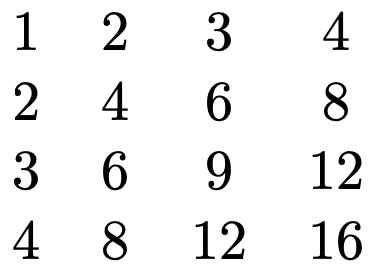
\includegraphics[width=0.4\linewidth]{Algebra/imgs/Sumas_problema_Olimp_pERU}
		%\caption{_caption_}
		%\label{fig:_name_}
	\end{figure}	
	Exprese el resultado mediante una multiplicación.
\end{enumerate}
\newpage


\section{Ecuaciones }\label{section:ecuaciones}
Te has preguntado cómo comparaban pesos en la antigüedad? Ahora es sencillo, solo debemos poner los pesos en una pesa y ver el valor para poder comprar. Antes usaban la \textbf{balanza} (Como la de la Figura \ref{fig_balanza})

\begin{figure}[H]
	\centering
	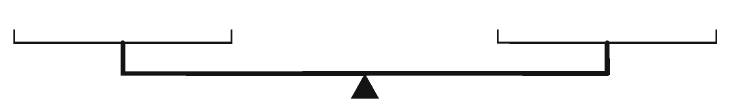
\includegraphics[width=0.6\linewidth]{Algebra/imgs/balanza_vacia.png}
	%	\caption{}
	\label{fig_balanza}
\end{figure}

Cuando pesan lo mismo se mantiene horizontal y cuando no, se inclina hacia el lado mas pesado.

\begin{tcolorbox}[colback=black!5!white,colframe=black]
	Mira este recurso en \textbf{modo básico} para aprender a usar una balanza:
	\begin{center}
		\url{https://phet.colorado.edu/es/simulation/equality-explorer-basics}.
	\end{center} 
	\textbf{Preguntas:}
	\begin{itemize}
		\item Si lograste equilibrar la balanza, es posible quitar frutas de forma de que siga equilibrada la balanza?
	\end{itemize}
\end{tcolorbox}

\begin{ejemplo}
	En la Figura \ref{fig_balanza2} se muestra una balanza equilibrada donde todos los bloques tienen un número que indican su peso. Hay un bloque que no tiene número, cuánto pesa?
	\begin{figure}[H]
		\centering
		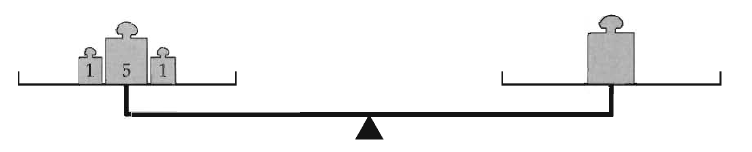
\includegraphics[width=0.8\linewidth]{Algebra/imgs/balanza_2.png}
		%	\caption{}
		\label{fig_balanza2}
	\end{figure}
	\textbf{Rta:} Pesa 7. Para la sigueinte balanza podemos representarlo con números con la siguiente ecuación:
	\[
		1+5+1=7
	\]
\end{ejemplo}

\begin{ejemplo} \label{ejemplo:balanza1_11}
	En la Figura \ref{fig_balanza1_11} se muestra una balanza equilibrada donde todos los bloques tienen un número que indican su peso en Kilogramos. 
	\begin{enumerate}[label=\Alph*)]
		\item Si cambiamos los bloques del plato derecho al plato izquierdo y los del izquierdo al plato derecho la balanza sigue equilibrada?
		
		\item Que ecuación representa esta balanza?
		
		\item Si agregamos 3kg en el lado derecho y 3 kg en el lado izquierdo permanecerá la balanza equilibrada?
		
		\item Al agregar estos pesos cuál sería la ecuación de la balanza?
		
		\item Suponga que ahora en vez de agregar, restamos 2Kg en el lado derecho y 2 kg en el lado izquierdo permanecerá la balanza equilibrada?
	\end{enumerate}

	\begin{figure}[H]
		\centering
		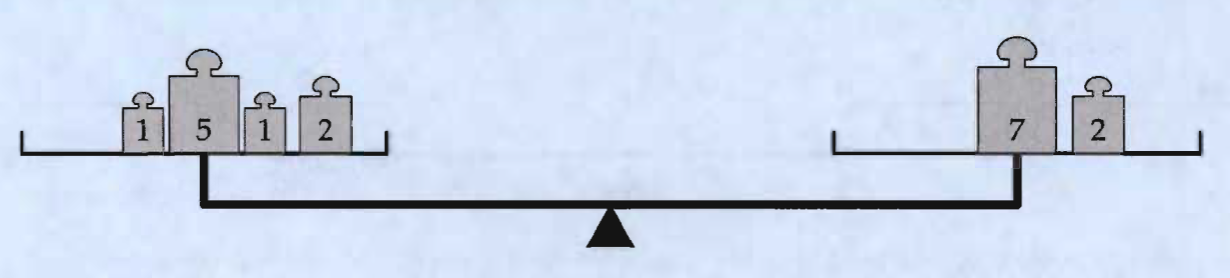
\includegraphics[width=0.8\linewidth]{Algebra/imgs/balanza1_11.png}
		\caption{Balanza del ejemplo \ref{ejemplo:balanza1_11}}
		\label{fig_balanza1_11}
	\end{figure}
\end{ejemplo}

\begin{ejemplo} 
	Supongamos que tenemos la ecuación
	\[
	17-7=9+1
	\]
	Es verdadera? o Falsa?. 
	\begin{enumerate}[label=\Alph*)]
		\item Supongamos que multiplicamos la ecuación por tres a ambos lados: $3\times (17-7)=3\times (9+1)$. Es esta ecuación verdadera?
		
		\item Supongamos que dividimos la misma ecuación por dos: $\frac{17-7}{2} = \frac{9+1}{2}$. Es esta ecuación verdadera?
	\end{enumerate}
	\textbf{Rta: } Pensandolo como bloques y una balanza todo tiene sentido, multiplicar bloques hace que siga equilibrada, y partir bloques también. Pero \textcolor{red}{Cuidado!} con dividir por cero.
\end{ejemplo}

\begin{tcolorbox}[colback=red!5!white,colframe=red!75!black]
	Con los anteriores ejemplos vemos que al sumar, restar, multiplicar y dividir ecuaciones estas permanecen igual. Tomemos tres números cualquiera $a,b,c$ y supongamos que se cumple que
	\[
	a=b
	\]
	Entonces lo que vimos es que 
	\begin{multicols}{4}
		\begin{itemize}
			\item $a+c = b+c$
			\item $a-c = b-c$
			\item $a\times c = b\times c$
			\item $\frac{a}{c} = \frac{b}{c}$
		\end{itemize}
	\end{multicols}
\end{tcolorbox}

\begin{ejemplo} 
	Tenemos la siguiente ecuación 
	\[
	\frac{73}{43}=\frac{511}{301}
	\]
	Es verdadera? o Falsa?.  Podemos convertir esta ecuación en esta otra $63\times 301 = 511 \times 43$ y así vemos que si es cierta.
\end{ejemplo}

\begin{exer}
Decir si las siguientes ecuaciones son verdaderas:
	\begin{multicols}{4}
		\begin{enumerate}[label= \Alph*)]
			\item $\frac{15}{30}=\frac{19}{38}$
			\item $\frac{8}{70}=\frac{4}{35}$
			\item $\frac{9}{8}=\frac{168}{112}$
			\item $\frac{33}{1703}=\frac{5}{258}$
		\end{enumerate}
	\end{multicols}
\end{exer}

\begin{tcolorbox}[colback=red!5!white,colframe=red!75!black]
	Con los anteriores ejemplos vemos que para cualesquiera cuatro números $a,b,c,d$ y supongamos que se cumple que
	\[
	\frac{a}{b} = \frac{c}{d}
	\]
	Entonces se cumple que 
	\[
	a\times d = c\times b
	\]
	A esto lo llamamos \textbf{multiplicación en cruz}.
\end{tcolorbox}


\begin{ejemplo}
		Suponga que se tienen las dos balanzas de la figura \ref{fig:2balanzas}.
		\begin{itemize}
			\item Representar las balanzas como ecuaciones.
			\item Si construimos una tercera balanza y juntamos las pesas de la izquierda de las balanzas en el lado izquierdo y las pesas derechas en el lado derecho, estará balanceada la nueva balanza?
			\item La diferencia de la parte izquierda de las ecuaciones es siepre igual a la diferencia de la parte derecha?
		\end{itemize}
		\begin{figure}[H]
			\centering
			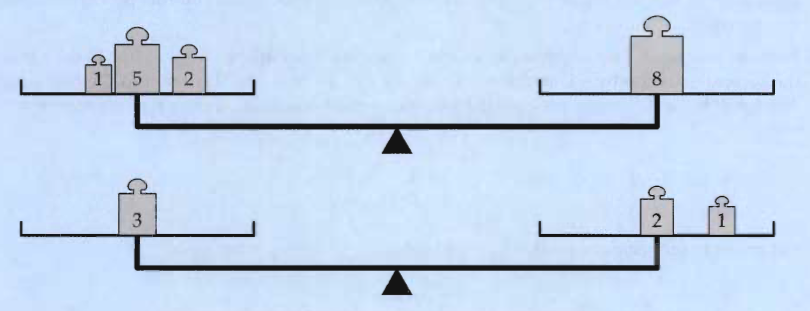
\includegraphics[width=0.8\linewidth]{Algebra/imgs/2balanzas.png}
			\caption{Dos balanzas}
			\label{fig:2balanzas}
		\end{figure}
\end{ejemplo}


\begin{tcolorbox}[colback=red!5!white,colframe=red!75!black]
	Con los anteriores ejemplos vemos que para cualesquiera cuatro números $a,b,c,d$ y supongamos que se cumple que
	\begin{align}
			a &= b\\
			c &= d
	\end{align}
	Entonces se cumple que 
	\[
	a+ c = b + d
	\]
	y también se cumple que 
	\[
	a - c = b - d
	\]	
\end{tcolorbox}

Que pasara si multiplicamos? Se seguirá cumpliendo? Has ejemplos.

\begin{tcolorbox}[colback=red!5!white,colframe=red!75!black]
	Con los anteriores ejemplos vemos que para cualesquiera cuatro números $a,b,c,d$ y supongamos que se cumple que
	\begin{align}
	a &= b\\
	c &= d
	\end{align}
	Entonces se cumple que 
	\[
	a\times c = b \times d
	\]

\end{tcolorbox}

\newpage

\begin{center}
	\vspace{-1cm}
	\subsection{ Ejercicios: Ecuaciones}\label{ejercicios:ecuaciones}
\end{center}

\begin{enumerate}
	\item Todo número tiene un recíproco, por ejemplo, el recíproco de $2$ es $\frac{1}{2}$. Otro ejemplo: el reciproco de $13$ es $\frac{1}{13}$. Si se tiene una ecuación, será que los reciprocos de cada lado de la ecución son iguales?
	
	\item Suponga que tiene dos ecuaciones cualquiera, por ejemplo
		\begin{align}
	a &= b\\
	c &= d
	\end{align}
	Será que siempre se cumple que $\frac{a}{c} = \frac{b}{d}$? 
	
\end{enumerate}
\newpage

\begin{center}
	\vspace{-1cm}
	\subsection{ Juego: Ecuaciones}
\end{center}
\begin{tcolorbox}[colback=yellow!15!white,colframe=black]
	\textbf{Juego: }\\
	Se empieza con un grupo de números y la idea es usar operaciones y paréntesis para formar el número 24. Por ejemplo
	si empezamos con el grupo:
	\[
	2,3,6,6
	\]
	Mi solución puede ser:
	\[
	(6+ 2)\times (6-3) = 24
	\]
	Yo como profesor los reto a ustedes a que lo logren con cada uno de los siguientes grupos:
		\begin{multicols}{3}
		\begin{itemize}
			\item 1,2,6,9
			\item 4,6,8,8
			\item 4,5,6,8
			\item 1,3,6,8
			\item 6,8,8,9
			\item 1,3,4,7
			\item 3,3,7,7
			\item 1,5,5,5
			\item 1,3,4,6									
		\end{itemize}
	\end{multicols}

		Si los lograste todos, crea tú un reto, elige un grupo de numeros, forma el 24 y reta a un amigo con el grupo que elegiste a ver si el es capaz de formar el 24.
\end{tcolorbox}



\chapter{X es la clave}\label{chapter:reglasAritmeticas}

\section{Expresiones}\label{section:expresiones}
Las expresiones las podemos encontrar en muchas circunstancias, veamos algunos ejemplos.

\begin{ejemplo}
	Supongamos que la temperatura de Cartagenta siempre es 10 grados mas que la temperatura en bucaramanga, entonces una expresión para calcular la temperatura en bucaramanga es 
	\[
	\underbrace{\rule{10mm}{0.15mm}}_{\text{Temperatura buaramanga}} + 10 
	\]
\end{ejemplo}

\begin{tcolorbox}[colback=black!5!white,colframe=black]
	\textbf{Aplicando a programación:}
	Para el anterior ejercicio se puede usar \textbf{Scratch} para crear un muñeco que le digamos la temperatura en bucaramanga y nos diga la temperatura en Cartagena.
\end{tcolorbox}

\begin{ejemplo}
	Suponga que queremos calcular el área de un rectángulo entonces la expresión para hacerlo es 
	\[
	\underbrace{\rule{10mm}{0.15mm}}_{\text{Lado}} \cdot \underbrace{\rule{10mm}{0.15mm}}_{\text{Alto}}
	\]	
\end{ejemplo}

\begin{tcolorbox}[colback=black!5!white,colframe=black]
	\textbf{Aplicando a programación:}
	Para el anterior ejercicio se puede usar \textbf{Scratch} para crear un muñeco que le digamos el lado y la altura de un rectángulo y el nos diga el área del rectángulo
\end{tcolorbox}


\begin{ejemplo}
	Supongamos que la temperatura de Cartagenta siempre es 10 grados mas que la temperatura en bucaramanga, entonces si asginamos una letra $b$ para denotar la temperatura en bucaramanga, entonces la temperatura en cartagena es 
	\[
	b + 10 
	\]
	Por ejemplo, si la temperatura en bucaramanga es $25$ grados ($b=25$) entonces la temperatura en Cartagena es $35$ grados ($b+10=25+10$).
\end{ejemplo}

\begin{ejemplo}
	Suponga que queremos calcular el área de un rectángulo donde la medida de su lado es  $l$ y alto $a$, entonces el área del rectángulo es
	\[
	\text{Área del rectánguloes:  }l\cdot a
	\]	
	Por ejemplo si un rectángulo tiene $3m$ de lado ($l=3m$) y $5m$ ($a=5m$) de alto, entonces el área es $15m^2$ ($l\cdot a=3m \cdot 5m$).
\end{ejemplo}

\begin{ejemplo} (p.13 \cite{Dimensions_Math_6B}). Sara es 7 años mayor que su hermano Tomás. Si consideramos que la edad de tomás es $t$ años,
	\begin{enumerate}[label=\Alph*)]
		\item escriba una expresión para expresar la edad de Sara en términos de $t$.
		\item Cuántos años tendrá Sara cuando Tomás tenga 32 años?
	\end{enumerate}
\end{ejemplo}

\begin{exer} (p.14 \cite{Dimensions_Math_6B})
	Nicolás es 4 años mayor que su hermana María. Si consideramos que la edad de María es $m$ años,
	\begin{enumerate}[label=\Alph*)]
		\item escriba una expresión para expresar la edad de Nicolás en términos de $m$.
		\item Cuántos años tendrá Nicolás cuando María tenga 20 años?
	\end{enumerate}		
\end{exer}

\begin{ejemplo} (p.16 \cite{Dimensions_Math_6B})
	En una escuela hay 3 veces más niños que niñas. Sabiendo que el número de niñas es $g$,
	\begin{enumerate}[label=\Alph*)]
		\item escriba una expresión para expresar el número de niños en términos de $g$.
		\item Si hay $12$ niñas en la escuela, cuántos niños hay?
	\end{enumerate}
\end{ejemplo}

\begin{exer} (p.16 \cite{Dimensions_Math_6B})
	En una venta de carros hay 4 veces más carros que camiones. Sabiendo que el número de camiones es $c$,
	\begin{enumerate}[label=\Alph*)]
		\item escriba una expresión para expresar el número de carros en términos de $c$.
		\item Si hay $55$ camiones, cuantos carros hay en la venta ?
	\end{enumerate}
\end{exer}

\begin{ejemplo} Reemplazar en cada espacio en blanco de las sigueintes expresiones el número 4.
	\begin{multicols}{2}
		\begin{enumerate}[label=\Alph*)]
			\item $\frac{(\rule{5mm}{0.15mm} + 12 )}{\rule{5mm}{0.15mm}}$
			\item ${(\rule{5mm}{0.15mm})}^2 + 2$
		\end{enumerate}
	\end{multicols}
\end{ejemplo}

\begin{exer} Reemplazar en cada espacio en blanco de las sigueintes expresiones el número 5.
	\begin{multicols}{2}
		\begin{enumerate}[label=\Alph*)]
			\item $\frac{(\rule{5mm}{0.15mm} -5  )}{3 \rule{5mm}{0.15mm}}$
			\item $3 {(\rule{5mm}{0.15mm})}^2 $
			\item $ {(\rule{5mm}{0.15mm})}^3 $
			\item $\frac{(3 \rule{5mm}{0.15mm}  )}{5}$
		\end{enumerate}
	\end{multicols}
\end{exer}

\begin{ejemplo} Evaluar cada una de las siguientes expresiones cuando $x=6$
	\begin{multicols}{2}
		\begin{enumerate}[label=\Alph*)]
			\item $x+3$
			\item $x^2 + 3$
		\end{enumerate}
	\end{multicols}
\end{ejemplo}

\begin{exer} Evaluar cada una de las siguientes expresiones cuando $x=6$
	\begin{multicols}{2}
		\begin{enumerate}[label=\Alph*)]
			\item $2x$
			\item $\frac{x+12}{x}$
			\item $3x^3$
			\item $\sqrt{5x-5}$
		\end{enumerate}
	\end{multicols}
\end{exer}

\newpage

\begin{center}
	\vspace{-1cm}
	\subsection{ Ejercicios: Expresiones}\label{ejercicios:expresiones}
\end{center}

\begin{enumerate}
	\item (p. 34 \cite{Aops_algebra}). Evaluar cada una de las siguientes expresiones cuando $r=3$
	\begin{multicols}{2}
		\begin{enumerate}[label=\Alph*)]
			\item $r-7$
			\item $-3r$
			\item $\sqrt{r^2 - {(r+1)}^2}$
			\item $\frac{5r}{3} - \frac{9}{r}$
		\end{enumerate}
	\end{multicols}
	
	\item (p. 34 \cite{Aops_algebra}). Evaluar cada una de las siguientes expresiones cuando $s=-4$
	\begin{multicols}{2}
		\begin{enumerate}[label=\Alph*)]
			\item $13-s$
			\item $\sqrt{-9s}$
			\item $-s^2 +4 -12$
			\item $\frac{s-8}{3}$
		\end{enumerate}
	\end{multicols}
	
	\item (p.17 \cite{Dimensions_Math_6B}). Evaluar cada una de las siguientes expresiones cuando $x=\frac{3}{4}$
	\begin{multicols}{2}
		\begin{enumerate}[label=\Alph*)]
			\item $4x+3$
			\item $\frac{2}{3}x-\frac{1}{4}$
			\item $0.5 + 12x$
			\item $\frac{1}{x} + \frac{5}{3}$
		\end{enumerate}
	\end{multicols}
	
\end{enumerate}
\newpage

\section{Aritmética con expresiones}\label{section:aritmeticaConExpresiones}

\begin{ejemplo}
	Juan tiene 5 legos y Valentina tiene 3 legos. Suponga que cada lego tiene $x$ fichas:
	\begin{enumerate}[label=\Alph*)]
		\item Escriba una expresión para saber la cantidad de fichas que tiene Juan y la cantidad de fichas que tiene Valentina.
		
		\item Cuantas fichas tienen entre ambos?
		
		\item Cuánto es $5x+3x$?
		
		\item Cuánto es $12x + 10x$?
		
		\item Cuánto es $3y + 7y$?
	\end{enumerate}
\end{ejemplo}

\begin{tcolorbox}[colback=red!5!white,colframe=red!75!black]
	Si tenemos términos iguales podemos sumarlos o restarlos, por ejemplo
	\[
	2x+3x+4x=9x
	\]
	esto ocurre pues 
	\[
	2x+3x+4x=(2+3+4)\cdot x = 9\cdot x
	\]
	Podemos restarlos, por ejemplo
	\[3a-2a=a\]
	Algo que \textbf{no} podemos hacer es por ejemplo
	\[2x+3\neq 5x\]
\end{tcolorbox}

\begin{exer}
	Simplificar las siguientes expresiones:
	\begin{multicols}{2}
		\begin{enumerate}[label=\Alph*)]
			\item $3x+2x$
			\item $8y-2y$
			\item $a+a+a+a$
			\item $2y+y+4y$
			\item $\frac{1}{2}x + \frac{5}{2}x$
			\item $s + \frac{1}{2}s$	
		\end{enumerate}
	\end{multicols}
\end{exer}

\begin{ejemplo}
	Lisa tiene 4 cajas de barras de chicle y 5 barras de chicle extra. Natalia tiene 7 cajas de barras de chicle y 3 barras de chicle extras. Suponga que cada caja tiene $x$ barras de chicles
	\begin{enumerate}[label=\Alph*)]
		\item Escriba una expresión para saber la cantidad de barras de chicles que tiene Lisa.
		
		\item Escriba una expresión para saber la cantidad de barras de chicles que tiene Natalia.
		
		\item Escriba una expresión para saber la cantidad de barras de chicles que tienen entre Lisa y Natalia?
		
		\item Simplificar la expresión $(4x+5) + (7x+3)$.
		
		\item Simplificar la expresión $(3r-2) + (3r-4) + (7-5r)$.
	\end{enumerate}
	
	\textbf{Rta:} Entre ambas tienen 11 cajas y 8 barras, entonces en total tienen $11x+8$. Sabemos entonces que $(4x+5) + (7x+3) = 11x+8$, pero por que? Si asociamos y sumamo sterminos iguales podemos ver que es cierto. 
\end{ejemplo}

\begin{ejemplo}
	A Pedrito le pidieron simplificar la sigueinte expresión
	\[(3r-2) + (3r-4) + (7-5r)\]
	y su solución fue la siguiente
	\[3r+3r+5r +2-4+7\]
	que opinas de la solución de Pedrito?
	
	\textbf{Rta:} Hay dos errores.
\end{ejemplo}

\begin{exer}
	Simplificar las siguientes expresiones:
	\begin{multicols}{2}
		\begin{enumerate}[label=\Alph*)]
			\item $7x-3x+2$
			\item $15+y-y$
			\item $12+3x-x$
			\item $3s+4+2s-1$
			\item $8+2y-4-y$
			\item $4n+8-n+10$
		\end{enumerate}
	\end{multicols}
\end{exer}

\begin{tcolorbox}[colback=red!5!white,colframe=red!75!black]
	Si multiplicamos dos potencias que tienen la misma base entonces sus exponentes se suman, por ejemplo
	\begin{itemize}
		\item $2\cdot 2\cdot 2\cdot 2 = 2^4$
		\item $3^4\cdot 3^6 = 3^{10}$.
		\item $2\cdot 2\cdot 2\cdot 5\cdot 5\cdot 5\cdot5 =2^3\cdot5^4$
	\end{itemize}
\end{tcolorbox}

\begin{tcolorbox}[colback=red!5!white,colframe=red!75!black]
	Si dividimos una potencia sobre otra que tenga la misma base entonces sus exponentes se restan, por ejemplo
	\begin{itemize}
		\item $\frac{2^7}{2^3} = 2^4$
		\item $\frac{3^5}{3^3}= 3^2$.
		\item $\frac{7^{11}}{7^6} =7^5$
	\end{itemize}
\end{tcolorbox}

\begin{tcolorbox}[colback=red!5!white,colframe=red!75!black]
	La potencia de una potencia es el producto de los exponentes, por ejemplo 
	\begin{itemize}	
		\item ${(2^3)}^4=2^{12}$
		\item ${(3^2)}^5=3^{10}$
		\item ${(3^5)}^7=3^{35}$
	\end{itemize}
\end{tcolorbox}

\newpage

\begin{center}
	\vspace{-1cm}
	\subsection{ Ejercicios: Potencias}\label{ejercicios:potencias}
\end{center}

\begin{enumerate}
	\item En cada punto decir si las igualdades son verdaderas (V) o falsas(F).
	\begin{multicols}{2}
		\begin{enumerate}[label=\Alph*)]
			\item $5^2\times 5^3 = 5^{2+3}$
			\item $5^2\times 5^3 = 5^{2\times 3}$
			\item $5^2 + 5^3 = 5^{2+3}$
			\item ${(2^2)}^3 = 2^{2+3}$
			\item $5^3\times 6^3 = {(5\times6)}^3$
			\item $\frac{4^6}{4^3} = 4^{6\div 3}$
			\item $\frac{4^6}{4^3} = 4^{6-3}$
			\item $4^6 - 4^3 = 4^{6-3}$
			\item ${\left(\frac{8}{4}\right)}^3 = 3^{8\div 4}$
			\item $7^{2+3} = 7^2 \times 7^3$			
			\item $2^5\times 3^5 = 5^{2+3}$
			\item $4^2\times 2^2 = 2^{4+2}$
			\item $2^5 + 3^5 = {(2+3)}^5$
			\item ${(2^3)}^2 = 2^{3\times 2}$
			\item ${(5^3)}^2 = {(5^2)}^3$
			\item $\frac{6^4}{3^4} = 4^{6-3}$
			\item $\frac{5^4}{5^2} = 5^{4\div 2}$
			\item $\frac{6^4}{3^4}  = {{\left(\frac{6}{3}\right)}^4}$
			\item $8^2 - 3^2 = {(8-3)^2}$
			\item $7^{3\times 2} = {(7^3)}^2$
		\end{enumerate}						
	\end{multicols}
	
	\item Unir cada elemento de la columna izquierda (Desde (i) hasta (xv)) con alguno de la columna derecha (desde (a) hasta (o)).	
	\begin{multicols}{2}
		\begin{enumerate}[label=(\roman*)]
			\item $\frac{7^5}{7^2}$
			\item $\frac{5^7}{2^7}$
			\item $7^5\times 7^2$
			\item $5^7\times 5^2$
			\item ${(5^2)}^7$				
			\item ${(7^5)}^2$
			\item $5^7 \times 2^7$
			\item $2^5\times 7^5$
			\item $\frac{5^7}{5^2}$	
			\item $2^7\times 2^5$		
			\item ${(2^7)}^5$
			\item $7^2\times 5^2$
			\item $\frac{2^5}{7^5}$
			\item $\frac{7^2}{5^2}$
			\item $\frac{2^7}{2^5}$				
		\end{enumerate}
		\begin{enumerate}[label=(\Alph*)]
			\item $7^{(5-2)}$
			\item $2^{(7+5)}$
			\item $5^{(7+2)}$
			\item $7^{(5+2)}$				
			\item ${\left(\frac{5}{2}\right)}^7$
			\item $2^{7\times 5}$
			\item $7^{5\times 2}$
			\item $5^{(7-2)}$
			\item ${(2\times 7)}^5$
			\item ${\left(\frac{2}{7}\right)}^5$
			\item $5^{2\times 7}$
			\item ${(7\times 5)}^2$
			\item ${\left(\frac{7}{5}\right)}^2$
			\item $2^{(7-5)}$
		\end{enumerate}						
	\end{multicols}
	
	\item Usando las propiedades vistas simplificar lo que más se pueda.
	\begin{multicols}{2}		
		\begin{enumerate}[label=(\Alph*)]
			\item $11^3\times 11^4$
			\item ${(18^4)}^3$
			\item $\frac{7^6}{7^4}$
			\item $2^2\times 2^5\times 2^6$
			\item ${(7^2\times 7^3)}^5$
			\item $\frac{5^4\times 5^5}{5^6}$
			\item $7^4\times 11^2 \times 11^5\times 7^2$
			\item $\frac{3^6 \times 3^5}{2^4\times 2^5}$
			\item $\frac{17^5}{7^2\times 7^5\times 17^3}$
			\item $\frac{5^6}{5^3}$
			\item $6^3\times 6^4$
			\item ${(13^6)}^2$
			\item $\frac{2^5\times 2^6}{2^7}$
			\item $5^6\times 5^7\times 5^2$
			\item ${(5^6\times 5^2)}^3$
			\item $\frac{11^4}{11^2\times 5^2\times 5^3}$
			\item $17^2\times 11^4\times 17^3\times 11^5$
			\item $\frac{7^9\times 2^5}{2^4\times 7^2}$
		\end{enumerate}						
	\end{multicols}
\end{enumerate}
\newpage

\subsection{Aritmetica con potencias}
\begin{ejemplo}
	Resolver los siguientes ejercicios. 
	\begin{enumerate}[label=\Alph*)]
		\item Usar un exponente pra escribir $y\cdot y\cdot y$?
		
		\item \label{ej:pot_y}Simplificar el producto $y^2 \cdot y^4$.
		
		\item Simplificar el producto $(2x) \cdot 3x^3$.
		
		\item \label{ej:multiplicacionPotencia}Simplificar ${(v^3)}^5$ planteando a $v$ como una potencia simple.
		
		\item Simplificar ${(2x)}^3$ como una constante multiplicando a $v$ como una potencia simple.
	\end{enumerate}
	
	\textbf{Rta:} En el punto \textbf{\ref{ej:pot_y}} vemos que: el producto de potencias es sumar los exponentes, resolver por ejemplo:
	\[ a^4 \cdot a^5,\quad x^3\cdot x^{12}\]
	En el punto \textbf{\ref{ej:multiplicacionPotencia}} siguiendo la misma lógica podemos ver calcular
	\[{(x^2)}^4\]
\end{ejemplo}

\begin{exer}{\ \\}
	\begin{multicols}{2}
		\begin{enumerate}[label=\Alph*)]
			\item Simplificar $\frac{x^7}{x^3}$
			\item Simplificar $\frac{2x}{6}$
			\item Simplificar $\frac{6x^2}{x}$
			\item Simplificar $\frac{4x^9}{20x^2}$
		\end{enumerate}
	\end{multicols}
\end{exer}

\newpage
\begin{center}
	\vspace{-1cm}
	\subsection{ Ejercicios Sección: Aritmética con expresiones}
\end{center}	
\begin{enumerate}
	\item (p.43 de \cite{Aops_algebra}). Simplificar cada una de las siguientes expresiones
	\begin{multicols}{2}
		\begin{enumerate}[label=\Alph*)]
			\item $(3x-8) + (5x+7)$
			\item $(3-3x)+(-19x+27)$
		\end{enumerate}
	\end{multicols}
	\item (p.43 de \cite{Aops_algebra}). Simplificar cada una de las siguientes expresiones
	\begin{multicols}{2}
		\begin{enumerate}[label=\Alph*)]
			\item $t^3\cdot t^4$
			\item $(16x^2)(4x^5)$
			\item ${(y^5)}^9$
			\item ${(3x^2)}^6$
		\end{enumerate}
	\end{multicols}
	\item (p.43 de \cite{Aops_algebra}). Simplificar cada una de las siguientes expresiones
	\begin{multicols}{2}
		\begin{enumerate}[label=\Alph*)]
			\item $\frac{p^7}{p^2}$
			\item $\frac{25z^3}{30z^7}$
			\item $\frac{(4x^3)(2x^5)}{6x^4}$
			\item $\frac{24t^3}{15t^4} \cdot \frac{5t^8}{3t^6}$
		\end{enumerate}
	\end{multicols} 		
	
	\item (p.41 de \cite{Aops_algebra}). Simplificar cada una de las siguientes expresiones
	\begin{enumerate}[label=\Alph*)]
		\item $(2t-7) + (2t-7)$							
		\item $(2t-7) + (2t-7) + (2t-7)$
		\item $(2t-7) + (2t-7) + (2t-7)+ (2t-7)$	
	\end{enumerate}
	Nota algo interesante?
	\begin{enumerate}[resume,label=\Alph*)]
		\item \textbf{WOW}. Intenta simplificar la siguiente expresión
		\[\underbrace{(2t-7) + (2t-7) +\cdots +(2t-7)}_{\text{100 veces}}\]
	\end{enumerate}
	
	\item (p.41 de \cite{Aops_algebra}). Cuántas $r^4$ se tienen que multiplicar para obtener $r^{20}$?
	
	\item (p.41 de \cite{Aops_algebra}). Es esto correcto?
	\[\frac{5+3x}{x} = \frac{5+3\cancel{x}}{\cancel{x}}=5+3=8\]
	Si no, explique por qué no es correcto.
	
	\item \textbf{Bonus.} (p.41-42 de \cite{Aops_algebra}) Cuando tenemos $\frac{2^7}{2^5}$ vimos que es lo mismo que restar los exponentes y por tanto $\frac{2^7}{2^5}=2^2$. Pero que pasa si el exponente en el denominador es mas grande? Por ejemplo $\frac{2^3}{2^8}$, podemos ver que esto es lo mismo que $\frac{1}{2^5}$, pero si usamos la regla de restar los exponentes tenemos que $\frac{2^3}{2^8}=2^{3-8}=2^{-5}$. Como ambos resultados deben ser iguales, entonces sabemos que \[2^{-5} = \frac{1}{2^5}.\]
	\begin{enumerate}[label=\Alph*)]
		\item Entonces a que sería igual $5^{-3}$?
		\item Evaluar $3^{-1}$
		\item Evaluar $7^{-2}$
		\item Evaluar $x^{-4}$
		\item Evaluar $\frac{1}{3^{-2}}$
		\item Evaluar $\frac{2x^{-3}}{x^5}$
		\item Evaluar $\frac{4}{x^{-4}}$								
	\end{enumerate}
	
\end{enumerate}
\newpage

\section{Distribución, substracción y factorización}\label{section:distribucion_substraccion_factorizacion}

En \ref{subsubsection_distributiva} vimos la propiedad distributiva y su factorización, es decir su forma inversa.

\begin{ejemplo}{\ \\}
	\begin{multicols}{2}
		\begin{enumerate}[label=\Alph*)]
			\item Expandir el producto $2(x+7)$
			\item Simplificar la expresión $2(x^2+3) + 3(x^2-9)$
		\end{enumerate}
	\end{multicols}
	\textbf{Sol: }Aplicar ley distributiva y luego agrupar terminos comunes.
\end{ejemplo}


\begin{ejemplo}{\ \\}
	\begin{enumerate}[label=\Alph*)]
		\item Mario y Carlos tienen dos serpientes de mascotas, la serpiente de Mario mide $7m$ y $7cm$, y la de Carlos $5m$ y $3cm$. Cúanto mas larga es la serpiente de Mario que la de Carlos?
		\item Simplificar la expresión $(x+3) - (3x+9)$.
		\item Simplificar la expresión $(t^2-5t+4)-(t^2-7)$.
	\end{enumerate}
	\textbf{Solución }
	\begin{enumerate}[label=\Alph*)]
		\item Rapidamente sabemos que la diferencia es de $7-5=2m$ y $7-3=4cm$. Esta es la ley distributiva
		\begin{align*}
		(7m+7cm) - (5m+3cm) &= 7m +7cm + (-1)(5m+3cm)\\
		&= 7m +7cm -5m-3cm\\
		&=(7m-5m)+(7cm-3cm)\\
		&=2m+4cm.
		\end{align*}
		\item Recuerde cómo distribuir cuando hay un menos
		\begin{align*}
		(x+3) - (3x+9) &= (x+3) + (-1)(3x+9)\\
		&= (x+3) + (-1)(3x) + (-1)(9)\\
		&= x+3-3x-9\\
		&=-2x-6		
		\end{align*}
		\item $-5t+11$. Recuerde tener cuidado con los signos.
	\end{enumerate}
\end{ejemplo}

Vamos a hacer ahora lo contrario, extraer los términos comunes usando la propiedad distributiva.

\begin{ejemplo}{\ \\}
	\begin{enumerate}[label=\Alph*)]
		\item Factorizar el 3 afuera de $3x+6$ para escribirlo como el producto de 3 por una expresión.
		\item Factorizar $-15a^2+35$
		\item Escribir $3x^2+2x$ como el producto de $x$ y otra expresión.
		\item Factorizar $2a^3+16a^2-8a$ lo mas que pueda.
	\end{enumerate}
	\textbf{Solución }
	\begin{enumerate}[label=\Alph*)]
		\item Recuerde $3x+6=3\cdot x+3\cdot 2 = 3() x+2$.
		\item $5(-3a^2+7)$.
		\item Cuidado, es diferente $5x^2 + 6x^2=(5+6)x^2=11x^2$. En este caso las expresiones de las variables son diferentes,
		\[3x^2+2x=x\cdot(3x) + x\cdot (2) = x(3x+2)\]
		\item $2a(a^2+8a-4)$. Podemos probar si nos quedó bien, multiplicando $2a$ por $(a^2+8a-4)$ y nos debe dar $2a^3+16a^2-8a$.
	\end{enumerate}
\end{ejemplo}

\begin{ejemplo}{\ \\}
	Factorizar la expresión $n(2n+1) + 5(2n+1)$.\\
	\textbf{Solución: } $(n+5)(2n+1)$. Acá factorizamos una expresión: $2n+1$, si no lo ves usa colores, o figuras en vez de la expresión que quieres factorizar $n\triangle +5\triangle = (n+5)\triangle $.
\end{ejemplo}

\begin{exer}{\ \\}
	Usando una sustitución como la que hicimos con el tríangulo $\triangle $ intentar factorizar las siguientes expresiones:
	\begin{enumerate}[label=\Alph*)]
		\item $4(x^2+1)-x(x^2+1)$.
		\item $5r(r-1)-2(r-1)$.
		\item $3t\sqrt{t^2-t-1}+2\sqrt{t^2-t-1}$.
	\end{enumerate}
\end{exer}

\begin{ejemplo}{\textbf{Problema.} \\}
	Sara hizo un truco de magia con Santiago. Ella le dijo que pensara en un número par, que lo multiplicara por dos, le sumara 48, lo dividiera por 4, le restara 7, lo multiplicara por 2 y le restara el número original. Luego, ella le dice el resultado que debió obtener. Cuál numero le dijo Sara a Santiago?\\
	\textbf{Solución: }Como no sabemos el número de Santiago, diremos que pensó en un número $x$. Entonces siguiendo las instrucciones
	\begin{align*}
	\text{Número inicial }&=x\\
	\text{Multiplica por dos }&=2x\\
	\text{Sumar 48 }&=2x+48\\
	\text{Dividir por 4  }&=\frac{2x+48}{4}\\						
	\text{Restar 7  }&=\frac{2x+48}{4} - 7\\					
	\text{Multiplicar por 2}&=2\left(\frac{2x+48}{4} - 7\right) \\					
	\text{Restar el número original  }&=2\left(\frac{2x+48}{4} - 7\right)-x.
	\end{align*}
	De seguro Sara sabe simplificar todo esto
	\begin{align*}
	2\left(\frac{2x+48}{4} - 7\right)-x &= \left(2\cdot\frac{2x+48}{4} - 2\cdot 7\right)-x\\
	&=\left(\frac{2(2x+48)}{4} - 14\right)-x\\
	&= \left(\frac{2x+48}{2} - 14\right)-x\\
	&= \left(\frac{2(x+24)}{2} - 14\right)-x\\		
	&= (x+24)- 14-x\\				
	&=x+10-x\\
	&=10.
	\end{align*}
\end{ejemplo}

\newpage
\begin{center}
	\vspace{-1cm}
	\subsection{ Ejercicios: Distribución, substracción y factorización }
\end{center}	
\begin{enumerate}		
	\item Simplificar cada uno de los siguientes productos
	\begin{multicols}{2}
		\begin{enumerate}[label=(\Alph*)]
			\item $2(2t-7)$
			\item $x(x+9)$
			\item $(x^3 -2x^2 +x +1)\cdot (3x^2)$
		\end{enumerate}
	\end{multicols}
	\item Simplificar cada uno de los siguientes ejercicios
	\begin{multicols}{2}
		\begin{enumerate}[label=(\Alph*)]
			\item $(3x+7)-(4x+9)$
			\item $(r^2 +3r -2) - (r^2+7r-5)$
			\item $3(t+7)-t(t+9)$
		\end{enumerate}
	\end{multicols}
	\item Factorice cada uno de los siguientes ejercicios
	\begin{multicols}{2}
		\begin{enumerate}[label=(\Alph*)]
			\item $12a-18$
			\item $7x^2-30x$
			\item $-8t^2+4t+16$
			\item $9z^3 -27z^2 + 27z$
		\end{enumerate}
	\end{multicols}
	\item Yo tengo una maquina mágica. Si tu introduces un número en mi máquina mágica, la maquina le suma 8 al número, luego multiplica el resultado por 6, luego le resta 12 a ese resultado. La maquina luego divide ese resultado por 2, luego a esto le resta un número que es 18 más que el número original que se introdujo a la máquina.
	\begin{enumerate}[label=(\Alph*)]
		\item Haz un bosquejo de cómo funciona mi máquina. Luego, introduce en la máquina los números que tu quieras. Que parece que les está haciendo la máquina a los números que le estas introduciendo? 
		\item Para probar esto que descubriste en la parte (A), intenta introducir ahora $x$ en la máquina. Escribe la expresión que arrojará la máquina lo mas simplificado posible.
	\end{enumerate}
	
	\item Factorice la expresión $2x(x-3) + 3(x-3)$.
	
\end{enumerate}
\newpage


\section{Fracciones}\label{section:fracciones}
\begin{ejemplo}{\ \\}
	\begin{enumerate}[label=\Alph*)]
		\item Simplificar la fracción $\frac{6x+9}{12}$.
		\item Simplificar la fracción $\frac{7t^2+3t}{t}$.
		\item Simplificar la fracción $\frac{3x-6}{x^2-2x}$.		
	\end{enumerate}
	\textbf{Solución A)}. 
	\begin{align*}
	\frac{6x+9}{12} &= \frac{3\cdot (2x+3)}{3\cdot 4} \\
	&= \frac{\cancel{3}\cdot (2x+3)}{\cancel{3}\cdot 4} \\
	&= \frac{2x+3}{4}
	\end{align*}
	
	\textbf{Solución B)}. 
	\begin{align*}
	\frac{7t^2+3t}{t} &= \frac{t\cdot (7t+3)}{t} \\
	&= \frac{\cancel{t}\cdot (7t+3) }{\cancel{t}} \\
	&= 7t+3
	\end{align*}
	
	\textbf{Solución C)}. 
	\begin{align*}
	\frac{3x-6}{x^2-2x} &= \frac{3\cdot (x-2)}{x\cdot (x-2)} \\
	&=  \frac{3\cdot \cancel{(x-2)}}{x\cdot \cancel{(x-2)}}\\
	&= \frac{3}{x}
	\end{align*}
	
\end{ejemplo}

\begin{tcolorbox}[colback=red!5!white,colframe=red!75!black]
	\textbf{Factorizar} nos puede ayudar para simplificar cuanco trabajamos con variables.
\end{tcolorbox}

\begin{ejemplo}{\ \\}
	Escribir la siguiente expresión con un mismo denominador
	\[\frac{2}{3x} + \frac{3}{x}\]
	\textbf{Solución: }Normalmente cuando intentamos sumar por ejemplo $\frac{2}{3} + \frac{1}{2}$, lo que hacemos es igualar denominadores 
	\[\frac{2}{3} + \frac{1}{2} = \frac{2\times2}{3\times2} + \frac{1\times3}{2\times3} = \frac{4}{6} + \frac{3}{6} = \frac{7}{6}\],
	Con este problema haremos lo mismo,
	\[\frac{2}{3x} + \frac{3}{x} = \frac{2}{3x} + \frac{3\cdot 3}{x\cdot 3} = \frac{2}{3x}  + \frac{9}{3x} = \frac{2+9}{3x} = \frac{11}{3x} \]
\end{ejemplo}

\begin{ejemplo}{\ \\}
	Escribir cada una de las siguientes expresiones con el mismo denominador
	\begin{enumerate}[label=\Alph*)]
		\item $\frac{2}{x^3} + \frac{3x}{5}$.
		\item $\frac{4}{3y} - \frac{5-y}{5y^2}$.		
	\end{enumerate}
	\textbf{Solución A)}. 
	\begin{align*}
	\frac{2}{x^3} + \frac{3x}{5} &= \frac{2 \cdot 5}{x^3 \cdot 5} + \frac{3x \cdot x^3}{5\cdot x^3}\\
	&= \frac{10}{5x^3} + \frac{3x^4}{5x^3} \\
	&= \frac{10+3x^4}{5x^3}
	\end{align*}
	
	\textbf{Solución B)}. 
	\begin{align*}
	\frac{4}{3y} - \frac{5-y}{5y^2} &= \frac{4\cdot 5y}{3y\cdot 5y} - \frac{(5-y)\cdot 3}{(5y^2)\cdot 3}\\
	&= \frac{20y}{15y^2} - \frac{15-3y}{15y^2} \\
	&= \frac{20y-(15-3y)}{15y^2} \\
	&= \frac{20y-15+3y}{15y^2} \\
	&= \frac{23y-15}{15y^2}
	\end{align*}
	
\end{ejemplo}



\begin{ejemplo}{\ \\}
	Escribir la siguiente expresión como una sola fracción
	\[\frac{3}{s} - \frac{7s}{s+2}\]
	\textbf{Solución: }Asi como cuando intentamos sumar por ejemplo $\frac{2}{3} + \frac{1}{2}$, lo que hacemos es igualar denominadores a $3\times 2$. Con este problema haremos lo mismo, igualaremos el denominador a $s(s+2)$
	
	\begin{align*}
	\frac{3}{s} - \frac{7s}{s+2} &= \frac{3\cdot (s+2)}{s\cdot (s+2)} - \frac{7s\cdot s}{(s+2)\cdot s}\\
	&= \frac{3s+6}{s\cdot (s+2)} - \frac{7s^2}{s\cdot (s+2)} \\
	&= \frac{3s+6-7s^2}{s\cdot (s+2) } \\
	&= \frac{-7s^2+3s+6}{s\cdot (s+2)} \quad \text{Ordenamos los terminos}	
	\end{align*}
	
\end{ejemplo}


